\documentclass[11pt,a4paper]{article}
\usepackage{hyperref}
\usepackage{color}
\usepackage{amsmath, amsthm, amssymb, amsfonts, verbatim}
\usepackage{graphicx}
\usepackage[table,x11names]{xcolor}
\usepackage{geometry}
\usepackage{subcaption}
\usepackage[numbers]{natbib}

\title{Assessing paravascular transport in the parenchyma by PDE constrained optimization.}

\renewcommand{\comment}[1]{\textcolor{red}{#1}}

\newcommand{\kam}[1]{\textcolor{blue}{#1}}

\author{Lars Magnus Valnes, Sebastian K. Mitusch, Geir A. Ringstad, \\ 
Per Kristian Eide, Simon W. Funke, Kent-Andre Mardal }


\begin{document}
\maketitle

\begin{abstract}
bla bla 
\end{abstract}
\section{Introduction}
Recent breakthroughs in medicine have linked neurodegenerative diseases like Alzheimer's to insufficient sleep through a novel fluid mechanism called the glymphatic system 
that is responsible for waste clearance. 
In 2011,~\citet{iliff2012paravascular} discovered a novel system within our brain's metabolism system, which changed our understanding of the brain. 
The system involves a new pathway, called the paravascular pathway as it runs in parallel with vasculature system in a surrounding compartment.
The important novelty in the 2011 findings was that waste from the brain is cleared through the paravascular path, and that a malfunction of this system 
is linked to the development of dementia such as Alzheimer's and Parkinson's diseases. In 2013,~\citet{xie2013sleep} found
that this system is particularly active during sleep.
These mentioned breakthroughs were all performed in mice. In 2018,  
it was for the first time demonstrated the action of
this system in humans, and that the action of the system differs
between healthy controls and patients with dementia~\citet{ringstad2018brain}. 
However, the biomechanical mechanisms behind this is not well understood from a fluid mechanics perspective,
and so far the modeling attempts have mostly failed~\citet{asgari2016glymphatic, holter2017interstitial, smith2017glymphatic}. 
In particular the system seems to facilitate waste transport faster than  
the diffusion, which since the pioneering works of \citet{sykova2008diffusion} 
has been the prevailing paradigm. Here, we aim to investigate whether PDE constrained optimization can be used
to assess the effective diffusion coefficient on long time-scales (hours or days).   


%A novel pathway of the brain's metabolism system called the paravascular pathway, because it runs in parallel with 
%vasculature system in a surrounding compartment,  
%was discoved in 2011~\cite{iliff2012paravascular}. 
%%Later it was found that this system is particularly active during sleep~\cite{xie2013sleep}.  
%It has been proposed that this pathway plays an important role in the clearance of waste
%from the brain and hereby a malfunction of this system is linked to  the development of dementia such as Alzheimer's and Parkinson's diseases. That is, 
%the lymphatic system plays a crucial role in waste clearance in the rest of our body, but there are no lymph vessels inside
%the brain. As such, the metabolic process of the brain is not well understood and this is surprising since the brain is a very 
%energy demanding organ (about 10 times as demanding as the average organ). The circulatory system of the paravascular pathway 
%has therefore been named the glymphatic system~\cite{jessen2015glymphatic} as it has a similar role as the well-known lymphatic system and because the glia cells 
%are crucial in this system.  
%The glymphatic system remains controversial and modeling attempts
%has so far mostly failed to explain the biomechanics of the system~\cite{asgari2016glymphatic, holter2017interstitial, smith2017glymphatic}\kam{Lars: vi trenger flere her}. A proper biomechanical 
%understanding of the pathway has significant potential because
%dementia such as Alzheimer´s and Parkinson´s diseases are
%associated with accumulation of metabolic waste such as
%amyloid-beta and CSF-tau.  

In \cite{ringstad2018brain} brain-wide distribution of MRI-contrast was demonstrated during 24 hours after lumbar contrast injection. Brain-wide distribution by diffusion alone was deemed unlikely by the authors (some of which are co-authors). The argument was based on analytical considerations where it was calculated that 50\% contrast enrichment would occur after 
55 hours using the error function which is valid for planar diffusion. However, 
the surface of the brain is folded and is around five times larger than 
a corresponding surface of a ball with the same volume. Hence, 
a more rigorous modeling attempt is warranted. A complicating factor
is however that the contrast in the surrounding CSF is heterogenous
and changes significantly during the 24 hours of the investigations. 
Furthermore, images were obtained only at a few time-points during the investigations in \cite{ringstad2018brain}. As such the sparseness i times prevent a direct computation of the diffusion coefficients.

The pioneering works of Sykov{\'a} and Nicholson~\cite{sykova2008diffusion} demonstrated
that diffusion was a governing transport mechanism in the brain and estimated to be on the order
of $1.0e-4 \mathrm{mm\sp{2}/s}$ for large molecules. This is confirmed with DTI where values of young and healthy are typically around $0.7e-3 \mathrm{mm\sp{2}/s}$ \cite{Helenius194}
while values in dementia typically are XXX \kam{Geir vet du dette?}. Of course diffusion coefficient 
measured by DTI at a time-scale of 7-30 minutes, may not be representative for the process on a
longer time-scale, at least if the paravascular pathway plays an important role. The fact that the vasculature  occupy around 3\% of the brain volume 
and the paravascular network is substatantially smaller potentially render it invisible at the short time-scales of a DTI investigation 
while it may still be effective on longer time scales.   


Our purpose in this paper is to attempt a more rigorous methodology 
for assessing the apparent diffusion process where
the complex geometry of the brain is taken into account and time-scales of hours or days are taken into account. 
The approach we will take is to solve a PDE constrained optimization problem 
via adjoint methods where we have sparse observations on selected time-points, around 10 acquisitions during 24 hours. But through
the complete domain. Hence, the challenges faced from a mathematical point of view 
are that 1) the images are subject to noise, 2) resolution in space is limited to slightly less than (1 mm)$^3$ and 3)
the sparse observations through the time domain.  As such we need to assess the sensitivity of
the approach with respect important parameters such as to regularization parameters, noise levels and 
time resolution to determine whether this approach is a viable method
to obtain parameters involved time-scales. We remark that the purpose
of this paper is a systematic study of the mathematical challenges and that assessing  
whether clearance is governed by a process that is faster than diffusion is not the topic of the current paper. 

An outline of the paper is as follows. 
In Section 2 we present the methodology of the paper. Section 2.1-2.3 contains a detailed description of the medical imaging 
relevant to this study as we do not expect the reader to have prior knowledge of medical imaging. Section 2.4
describes the PDE constrained optimization problem and the corresponding solution algorithm, while 2.5 presents
a test problem using a manufactured solution that is used for method verification. Section 2.6 describes the implementation 
in FEniCS \cite{LoggMardalEtAl2012a}. In Section 3 we present the results and have a rather extensive discussion of the verification performed
using a manufactured solution (Section 3.1-3.3) before we present the results obtained by real observations in Section 3.4     
and a comparison with DTI data in Section 3.5. Finally, in Section 4, the methodology and results are discussed.  
   
\section{Methodology}

Section 2.1-2.3 describes the details of the imaging relevant for this study. More details can however be
found in e.g. \cite{ringstad2018brain}. Section 2.4-2.5 describe the solution of PDE constrained optimization problems and
its implementation in FEniCS. The exposition is, however, brief and we refer to XXX for more details. 







\subsection{MRI Data}
\begin{figure}
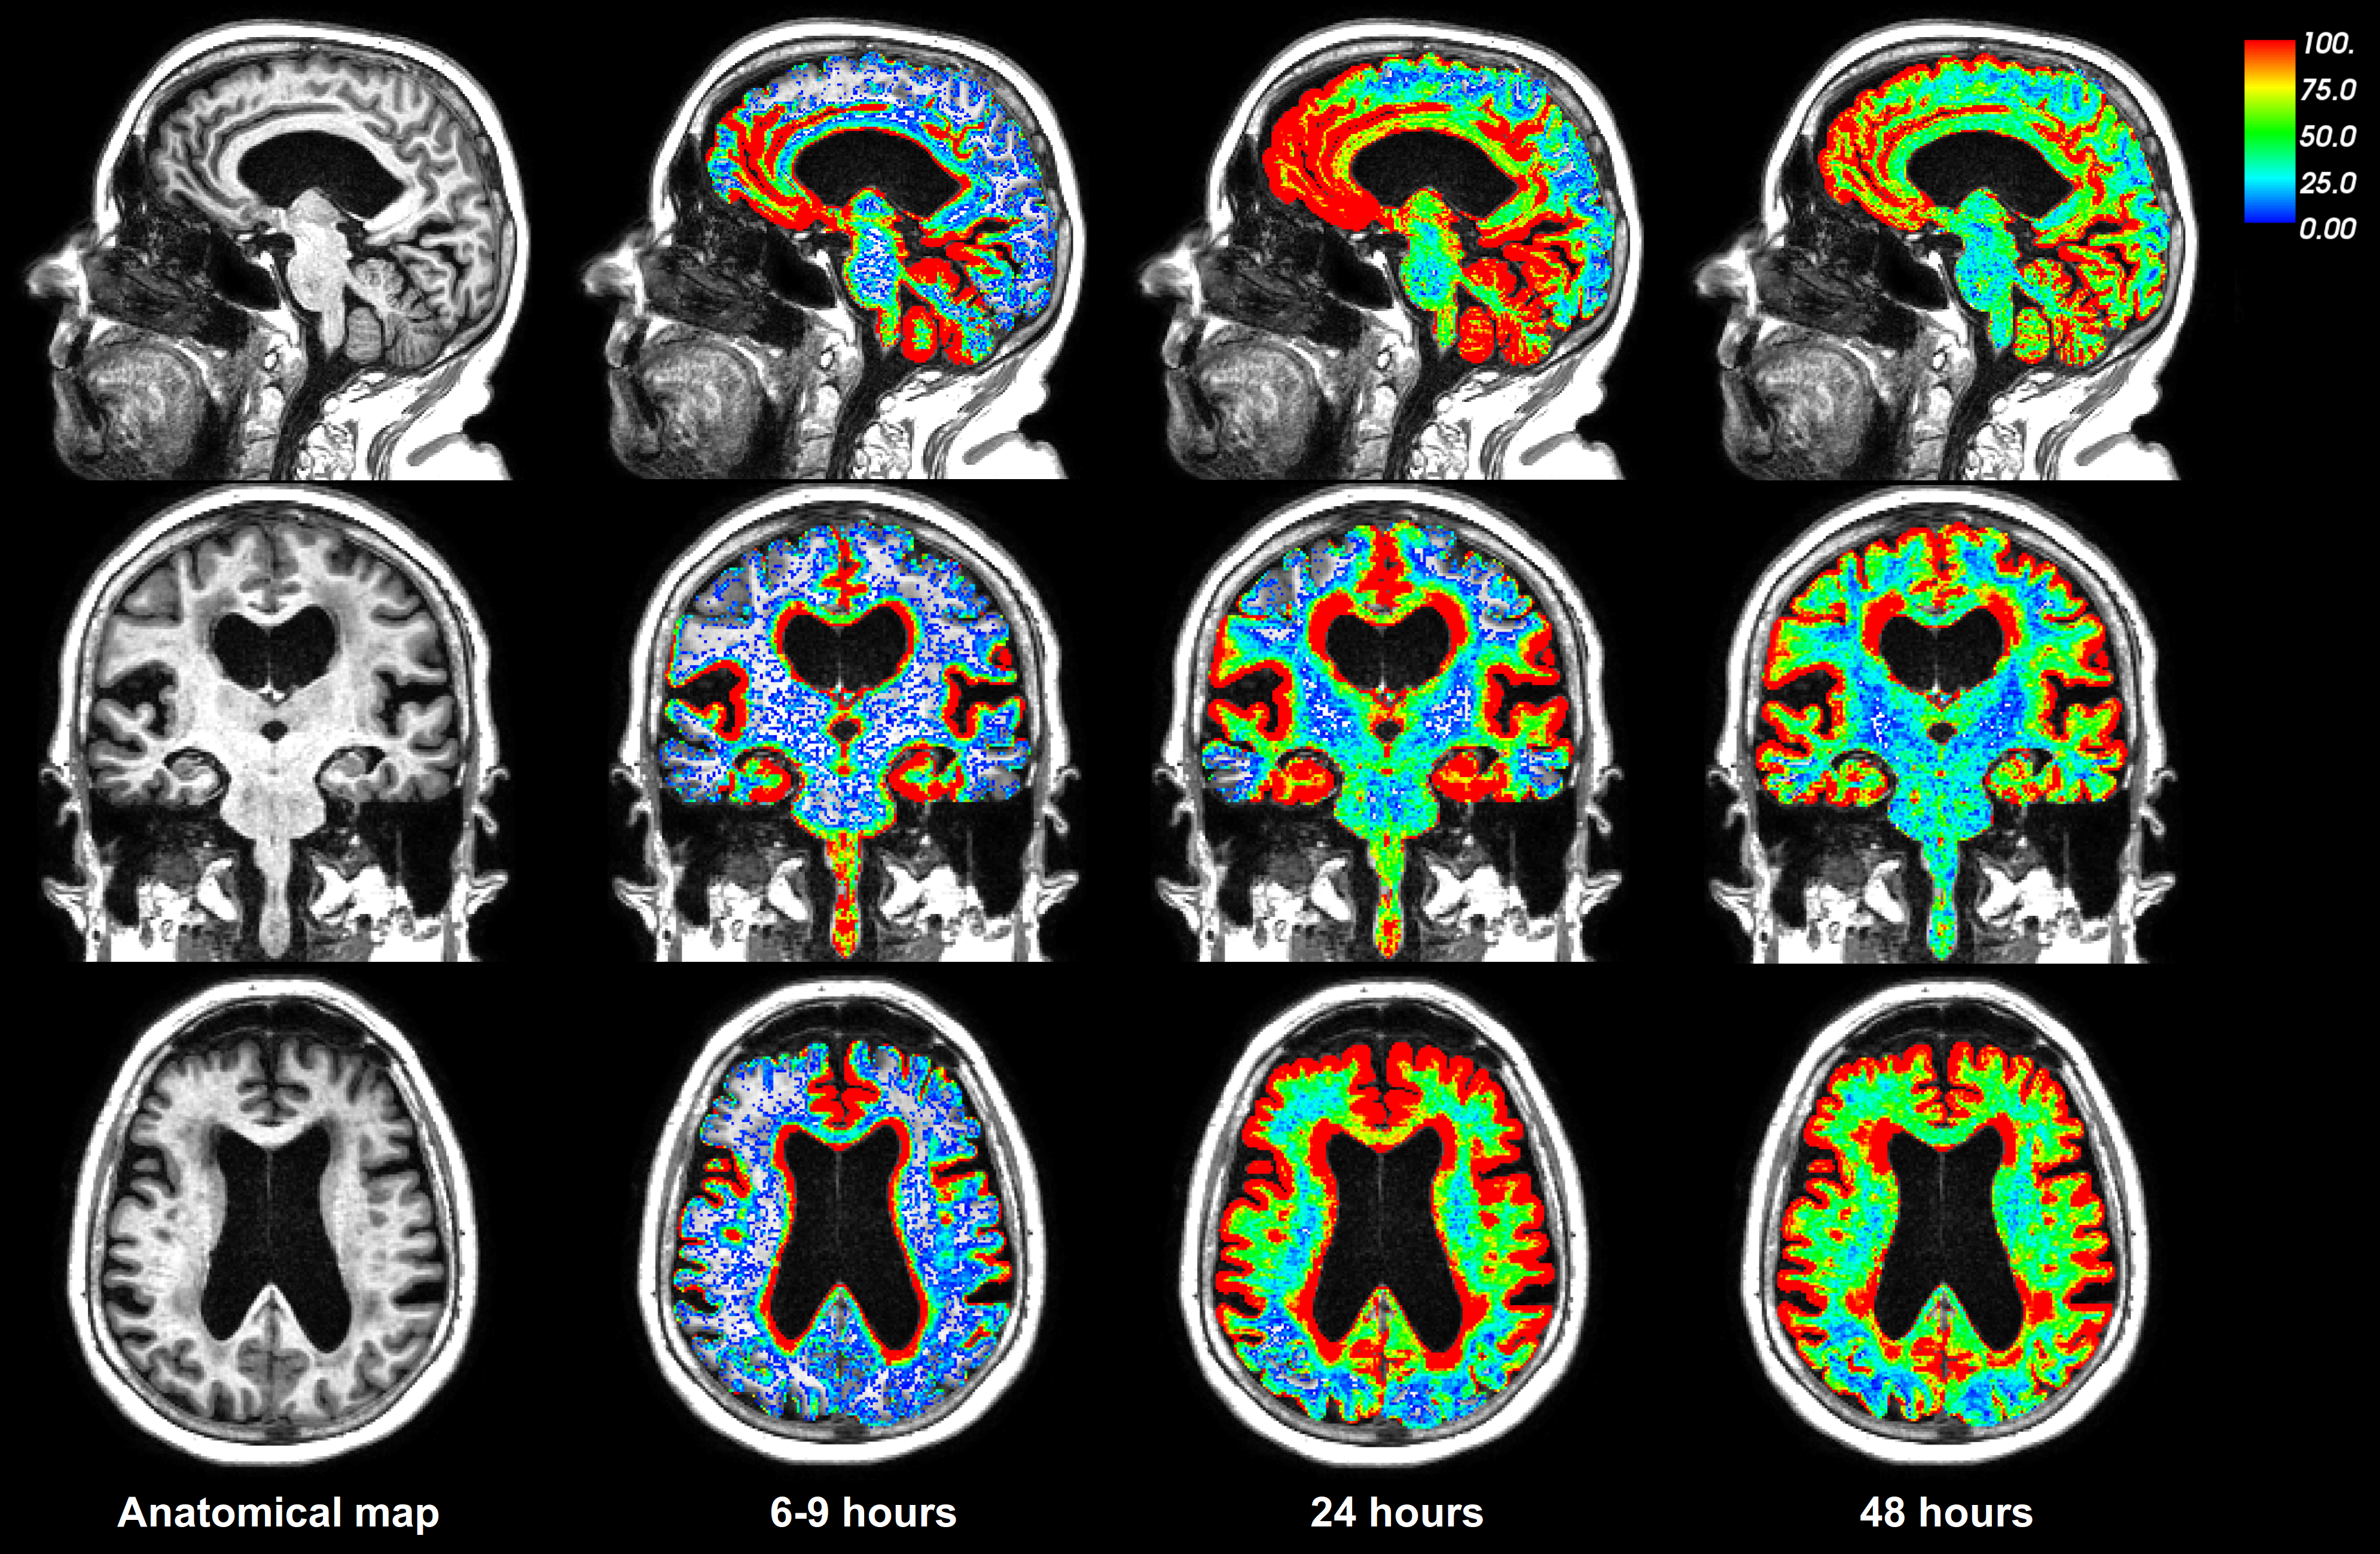
\includegraphics[width=0.95\textwidth]{PatID-68-new-100.png} 
\caption{Shows the percentage intensity increase from baseline at different observation times. The colorbar was restricted to the range $(0,100)$ }
\label{fig1} 
\end{figure}

\begin{figure}
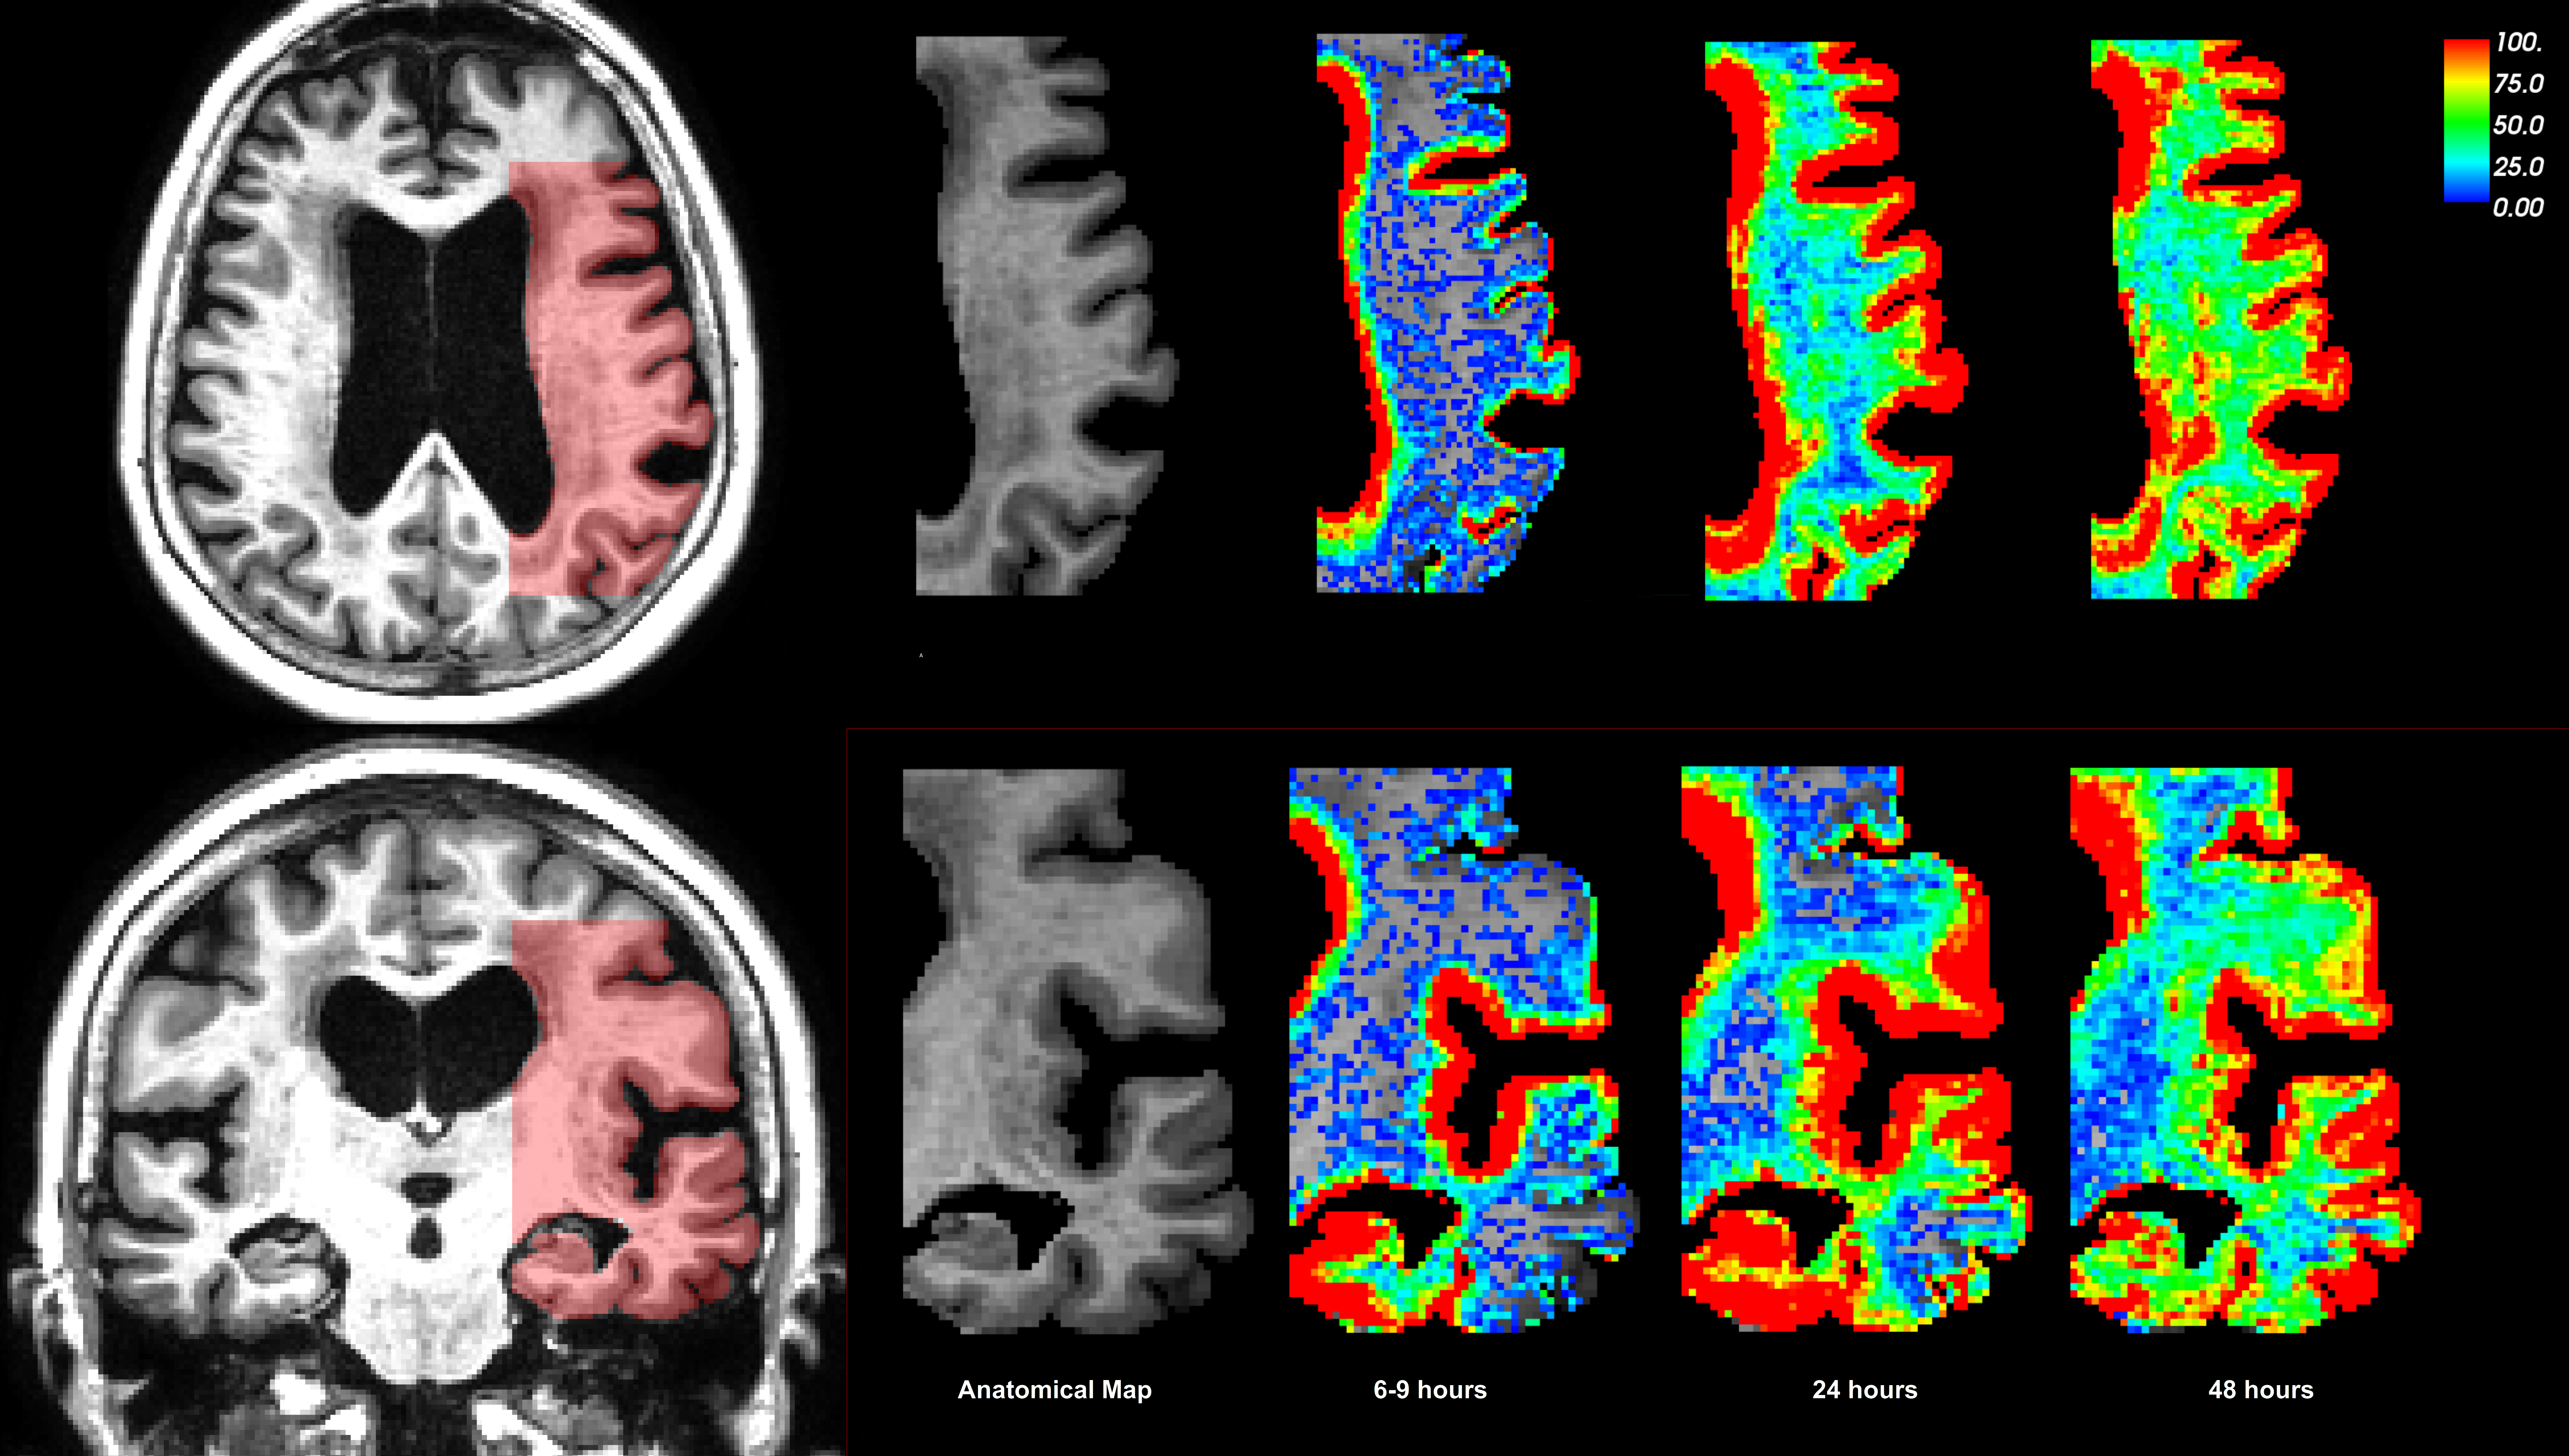
\includegraphics[width=0.95\textwidth]{Zoom-PatID-68.png} 
\caption{Shows the percentage intensity increase from baseline at different observation times in the slice (marked red in the left panel) used in the subsequent analysis.The colorbar was restricted to the range $(0,100)$}
\label{fig2} 
\end{figure}
Figure~\ref{fig1} shows the distribution of tracers during 24 hours, see also~\cite{ringstad2018brain} for further information on the imaging procedure.   
Our data (not all shown) consist of a total of 10 MRI observations, including a baseline MRI taken before tracer was injected. The observation points are distributed with 5 observations within 1-2 hours after injection, a single observation in the timeframes 2-4 hours, 6-9 hours, 24 hours and 48 hours. 
Figure~\ref{fig2} shows the region selected for our computations. 
The software Freesurfer \cite{Dale1999179, FischlLiuDale, spf2007, reuter:robreg10} was used to segment and align each of the observations, which made it possible to estimate voxelwise intensity increase. 

The MRI data is obtained from a larger study, which invloves around 100 patients with similar MRI acquisitions. However, due to the clinical factor, some of the parameters involved are different. Thus a thorough analysis is needed to obtain a robust and accurate method.

\subsection{Contrast concentration - Image Intensity Relation}
Below, we briefly describe the relationship between the imaging intensity 
seen in Figures \ref{fig1} and \ref{fig2} and the underlying contrast 
concentration. We remark that we use a notation common in medical literature and here two letter symbols are common. Hence, below we will use two letter symbols such as $TE$ and $TR$ to keep the notation consistent the presentation in \cite{GOWLAND, MPRAGE}.   
The tracer concentration $c$ causes the longitudinal(spin-lattice) relaxation time $T_{1}$ to shorten with the following relation
\begin{equation}
\frac{1}{T_{1}\sp{c}} = \frac{1}{T_{1}\sp{0}} + r_{1}c .
\label{EQ::contrast}
\end{equation}
The superscripts indicating with contrast $T_{1}\sp{c}$ and without contrast $T_{1}\sp{0}$ and $r_1$ as the relaxivity constant for the MRI tracer in a medium. 
The tracer observations were collected using a MRI sequence known as  Magnetization Prepared Rapid Acquisition Gradient Echo (MPRAGE) with an inversion prepared magnetization. The relation between intensity and the relaxation time is non-linear, and is expressed with the following equations. The signal intensity $S$ for this sequence is given by
\begin{equation}
S = M_{n} \sin \theta e\sp{ - TE/T_2\sp{*} },
\label{EQ::SI_T2}
\end{equation}
with $TE$ and $\theta$ respectively denoting the echo time and the flip angle, and $M_{n}$ the magnetization for the n-echo described below. 
Also $T_2\sp{*}$ is transverse magnetization caused by a combination of spin-spin relaxation and magnetic field inhomogeneity. It is defined as 
\begin{equation}
\frac{1}{T_2\sp{*}} = \frac{1}{T_2} + \gamma \Delta B_{in} ,
\end{equation}
with $T_2$ transverse (spin-spin) relaxation time, $\gamma$ is the gyromagnetic ratio and $\Delta B_{in}$ is the magnetic field inhomogeneity across a voxel. The expression can be simplified by neglecting the $T_2$ term in the signal, since $TE <<T_2\sp{*}$ for this MRI sequence. Thus \eqref{EQ::SI_T2} becomes 
\begin{equation}
S = M_{n} \sin \theta.
\label{EQ::SI}
\end{equation}
In article \cite{GOWLAND}, the term $M_n$ is defined as the magnetization for the n-echo 
\begin{equation}
M_{n} = M_{0}  \left[ (1-\beta)\frac{(1-(\alpha \beta)\sp{n-1} }{1-\alpha\beta} + (\alpha \beta)\sp{n-1}(1-\gamma) + \gamma ( \alpha \beta)\sp{n-1} \frac{M_{e}}{M_{0}}  \right]   
\end{equation}
with 
\begin{equation}
\frac{M_{e}}{M_{0}} = - \left[ \frac{ 1 -\delta + \alpha \delta (1-\beta ) \frac{1-\alpha\beta\sp{m}}{1-\alpha \beta} + \alpha\delta(\alpha\beta)\sp{m-1} - \alpha\sp{m}\rho}{1 +\rho \alpha\sp{m} } \right].
\end{equation}
Using the following definitions
\begin{equation}
\begin{aligned}
\alpha &= \cos ( \theta ) \\
\beta  &= e\sp{- \sp{T_b}/_{T_1\sp{0}} } \\
\delta &= e\sp{- \sp{T_a}/_{T_1\sp{0}} } \\
\gamma &= e\sp{- \sp{T_w}/_{T_1\sp{0}} } \\
\rho   &= e\sp{- \sp{TR}/_{T_1\sp{0}}}  \\
T_w    &= TR - T_a -T_b(m-1)       .\\
\end{aligned}
\end{equation}
Here $T_b$ is known as the echo spacing, $T_a$ is the inversion time, $T_w$ the time delay, $TR$ as the repetition time, $m$ is the number of echo spacings and $T1$ is the longitudinal(spin-lattice) relaxation time for a given medium. The $M_0$ is a calibration constant of the magnetization. The center echo denoted as $n=m/2$ will be the signal that we will consider when estimating MRI tracer. Given Eq.\ref{EQ::SI} we have that relative intensity increase can be written as 
\begin{equation}
\frac{S\sp{c}}{S\sp{0}} = \frac{ M_{n}\sp{c} \sin (\theta)}{ M_{n}\sp{0} \sin (\theta) } ,
\end{equation}
We define that  
\begin{equation}
f(T_1) = M_{n}/M_{0} ,
\label{scaledmagnetization}
\end{equation}
which can be seen in Figure () . 
This gives the following relation 
\begin{equation}
\frac{f(T_{1}\sp{c} ) }{f(T_{1}\sp{0})}  = \frac{S\sp{c}}{S\sp{0}} 
\end{equation}
The intensity difference between observation times were adjusted in \cite{eidevalnes}. Thus we can express the change in $T_1$ due to tracer as 
\begin{equation}
f ( T_{1}\sp{c} ) = \frac{S\sp{c}}{S\sp{0}} f(T_{1}\sp{0}) 
\end{equation}
and then estimate the concentration using \eqref{EQ::contrast}. The $T_{1}\sp{0}$ values were obtained by T1 mapping the brain using a MRI sequence known as MOLLI5(3)3 \cite{TAYLOR201667}. This takes into account patients specific characteristic, such as tissue damage. Tissue damage can be observed in the MRI due to a lower intensity in the white matter compared to healthy white matter tissue, thus damaged tissue have different $T_1$ relaxation time. 

\begin{figure}
\centering
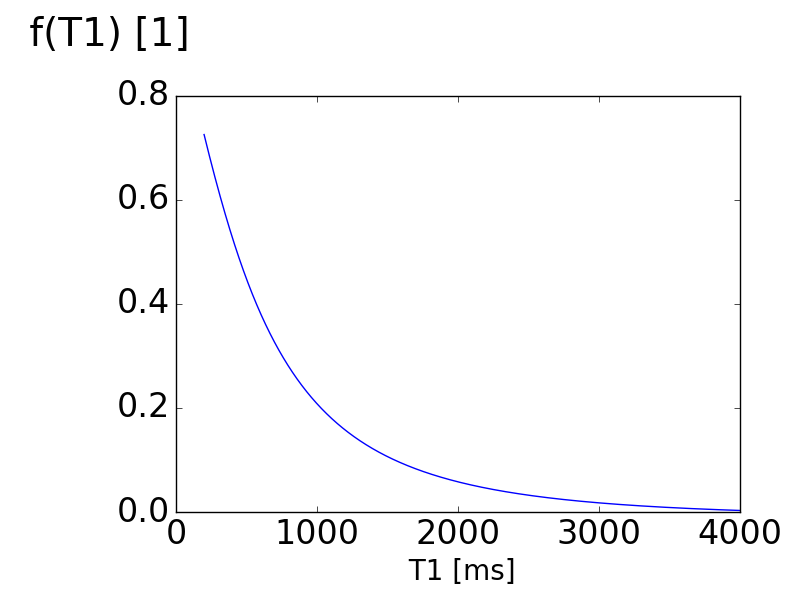
\includegraphics[width=0.70\textwidth]{T1function.png} 
\caption{Show the  function defined in \eqref{scaledmagnetization}. }
\label{figuredti} 
\end{figure}


\subsection{Diffusion tensor imaging}
In addition to the T1 and T2 weighted sequences described above we have also obtained diffusion tensor imaging (DTI) to assess the apparent diffusion 
coefficients on short time-scales. Images are shown in Figure~\ref{figuredti} where the larges diffusion coefficient (shown in 
red in the middle figure) is shown to be around $1.0e-3 mm^2/s$. We remark that we have not included possible anisotropy, shown in 
the right-most image in Figure~\ref{figuredti} and that these images shows the apparent diffusion coefficient for free water molecules (18 Da).      
The diffusivity of the Gadovist (600 Da \cite{MGadobutrol}) was estimated to be similar to the diffusion coefficient of Gd-DPTA (550 Da \cite{MGgDPTA}). This due to the fact that both molecules have similar mass, and based Stoke-Einstein equation should have similar diffusion coefficients. The free diffusion coefficient for Gd-DPTA was estimated in \cite{GdDPTA-DIFFUSION} to be $3.8e-4\mathrm{mm\sp{2}/s}$.
The fractional anisotropy is defined as 
\begin{equation}
FA\sp{2} =  \frac{3}{2} \frac{ (\lambda_1 - MD )\sp{2} +(\lambda_2 - MD )\sp{2} +(\lambda_3 - MD )\sp{2}}{\lambda\sp{2}_1 + \lambda\sp{2}_2  +\lambda\sp{2}_3 },
\end{equation}
with the mean diffusivity $MD$ defined as 
\begin{equation}
MD = \frac{\lambda_1 +\lambda_2 +\lambda_3 }{3}.
\end{equation}
In these equations $\lambda_i$ denotes the eigenvalues of the diffusion tensor.
\begin{figure}
\centering
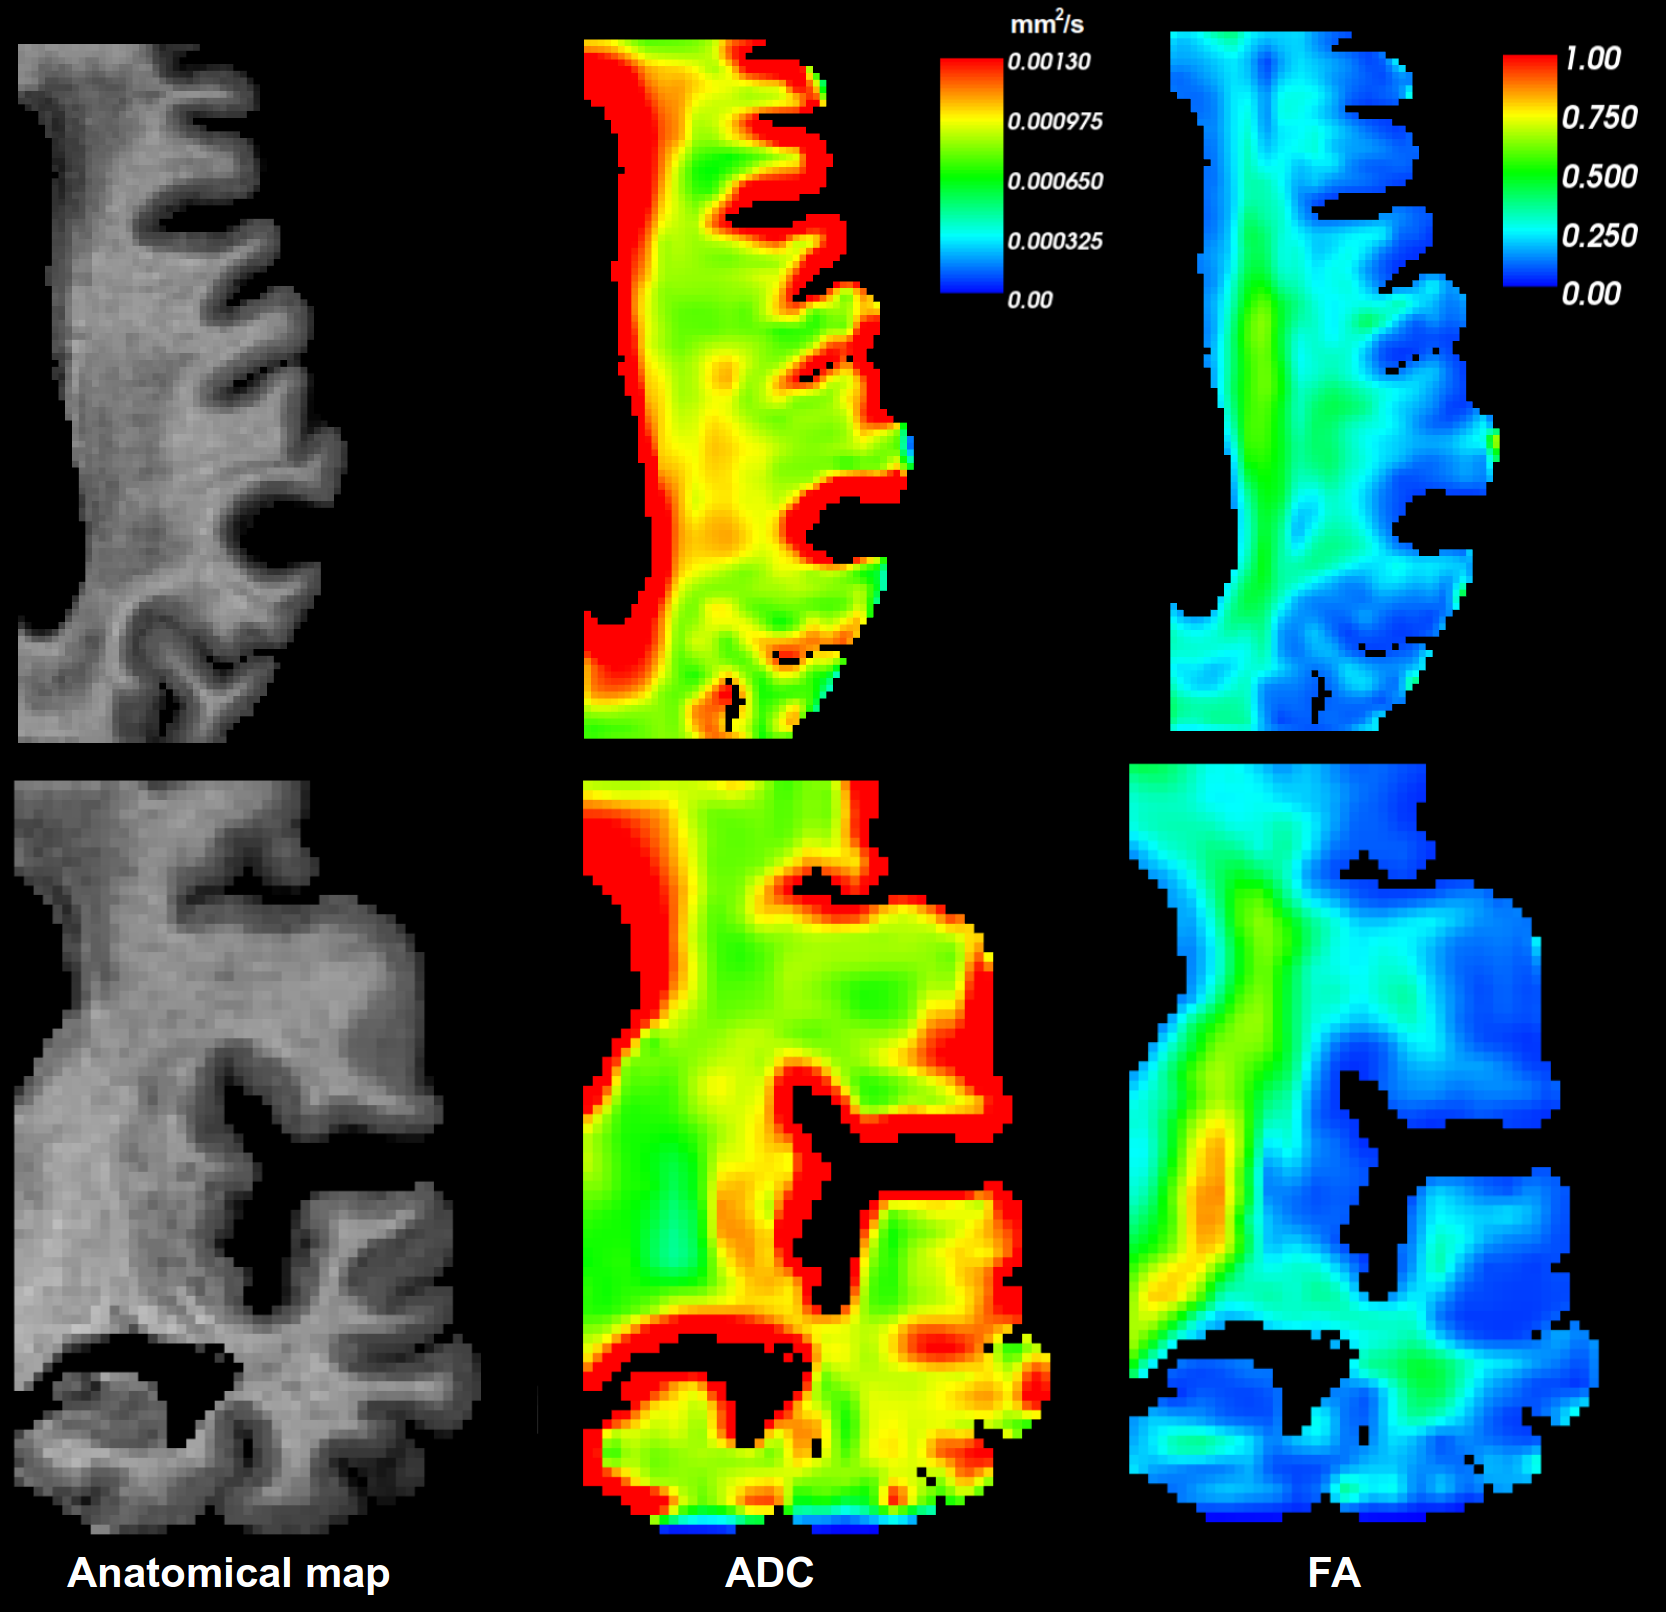
\includegraphics[width=0.80\textwidth]{DTI-zoom.png} 
\caption{The left panel show the anatomical map. The middle panel show the apparent diffusion coefficients (ADC) obtained from DTI. The right panel shows the computed fractional anisotropy (FA) from the DTI.}
\label{figuredti} 
\end{figure}


\subsection{Mathematical Model}
In \cite{sykova2008diffusion}, it was shown that the macroscopic diffusion in the brain can be considered a hindered diffusion with an apparent diffusion coefficient. In order to estimate the apparent diffusion coefficient involved in the tracer transportation shown in Figure~\ref{fig1} we assume that the process can be modeled by a diffusion equation. Then we solve a PDE constrained optimization problem where
the tracer distribution, boundary conditions, and apparent
diffusion coefficient are solved for by optimizing with
respect to the observed tracer distribution. As such, enhanced transportation because of effects such as
dissipation would result in an apparent diffusion coefficient larger than that predicted by DTI.  
The objective function was defined as 
\begin{equation}
\min_{D,g} F = \quad \sum\limits_i\sp{n} \int\limits_{\Omega} |u(t_i) - u_{obs}(t_i)|\sp{2} \mathrm{d}\Omega + \frac{\alpha}{2} \int\limits_{0}\sp{T} || g ||\sp{2}_{L\sp{2}(\partial\Omega)} \mathrm{d}t + \frac{\beta}{2} \int\limits_{0}\sp{T} || \dot{g} ||\sp{2}_{L\sp{2}(\partial\Omega)}\mathrm{d}t 
\label{EQ::objf}
\end{equation}
subject to   
\begin{equation}
\begin{aligned}
\frac{\partial u}{\partial t} = \nabla \cdot  D_i \nabla u \qquad \text{in} \qquad \Omega \times \left\lbrace 0 , T \right)  \\
u=g(t) \qquad \text{on} \qquad \partial\Omega  \times \left\lbrace 0 , T \right) 
\end{aligned}
\label{Eq::PDE}
\end{equation}
Here, $u$ is the contrast distribution, $D_i$ is the apparent diffusion 
coefficient, and $g$ is the boundary condition. Furthermore,  
the domain $\Omega$ contains three sub domains, each with a different diffusion coefficient. We denote the Cerebral Spinal fluid (CSF) domain as $\Omega_1$, the grey matter as $\Omega_2$ and the white matter as $\Omega_3$. The apparent
diffusion constant is assumed to be constant within the CSF, grey and 
white matter but each region may have different values.  
The $\alpha$ and $\beta$ parameters are non-negative regularization parameters 
and $u_{obs}$ are observations at certain time-points $t_i$. 

The mesh construction was patient-specific and used the MRI of a patient diagnosed with idiopathic normal pressure hydrocephalus (iNPH). The software Freesurfer was used in segmentation and creating the polyhedral surfaces of the white and grey matter. Then the use of T2 weighted MRI \cite{eidevalnes} was used to segment the CSF compartment surrounding the cerebral and the lateral ventricles. CGAL \cite{cgal:rty-m3-18b} was used to combine the polyhedral surfaces and to construed the mesh. The computational requirement for the resulting mesh was significant, therefore two submesh was also constructed, see Fig.\ref{Fig::Mesh}.
\begin{figure}
\centering
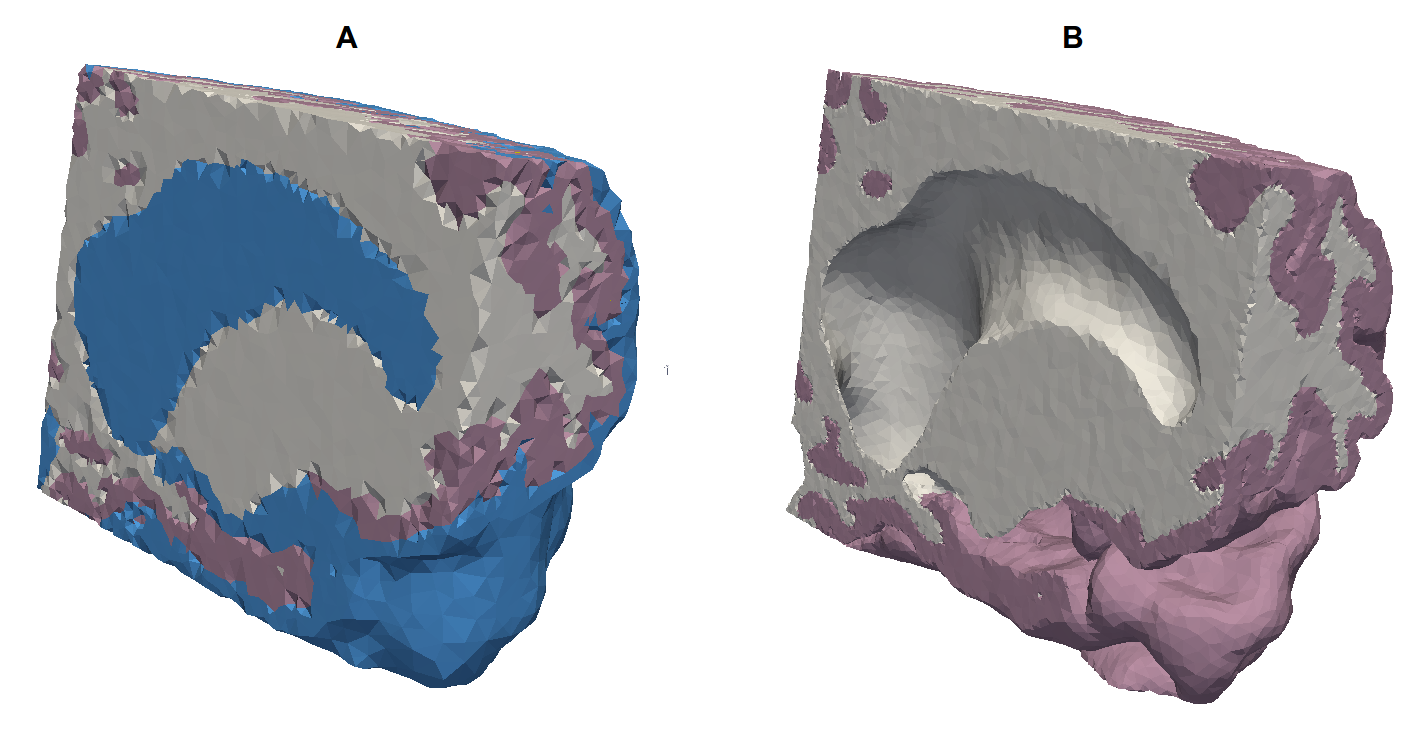
\includegraphics[scale=0.2]{mesh.png} 
\caption{A) Shows the mesh created from the baseline MR image with 3 domains. B) Shows the mesh created from the baseline MR image with 2 domains.  }
\label{Fig::Mesh}
\end{figure}
The 3 domain mesh in Fig.\ref{Fig::Mesh} A, consists of 244318 tetrahedral cells and 22057 vertices, while the 2 domain mesh Fig.\ref{Fig::Mesh} B consists of 335589 tetrahedral cells and 73002 vertices. The dimension of the mesh coordinates are $\mathrm{mm}$.


\subsection{Manufactured Solution}
In order to asses the robustness and accuracy of our strategy and test the dependency of the
regularization parameters, we perform a test case with a
known solution.  
The manufactured observations was obtained by forward computation of Eq.\ref{Eq::PDE} with the Dirichlet boundary condition defined as
\begin{equation}
g(t)_{\partial \Omega_1} = 0.3 +0.167t - 0.007t\sp{2} \qquad  0 \leq t \leq 24.
\label{EQ::DIRI}
\end{equation}
The timestep was $dt = 0.02$, and the diffusion coefficients were selected to be 
\begin{equation}
D_{\Omega_1} = 1000 \quad , \quad D_{\Omega_2} = 4.0 \quad , \quad D_{\Omega_3} = 8.0 
\end{equation}  
The magnitude order for $D_{\Omega_1} $ and $D_{\Omega_2}$ were chosen to resemble diffusion coefficient for water in grey and white matter, but the relation between the coefficients were not preserved. The diffusion coefficient in the CSF was chosen given [cite Bryne and Kent], and the initial condition was set to 0 everywhere. %and the initial condition was set to 1.0 in $\Omega_1$ and 0 elsewhere.
The manufactured forward computation gave a total of 120 possible observation times.


\section{Implementation}
The estimation of the tracer concentration was precomputed and used the parameters obtained from the T1 map, MPRAGE MRI protocol \cite{eidevalnes} and the value for $r_1$ found in \cite{pmid16230904}. In the computation, the function Eq.\ref{scaledmagnetization} was computed for $ T_1\in \lbrace 200, 4000 \rbrace$ creating a lookup table. The lookup table was utilized with the baseline intensity increase to estimate $T_1\sp{c}$, and then the concentration was computed using Eq.\ref{EQ::contrast}.  

%In the acquired data, the MPRAGE had a high signal to noise ratio and the T1 map had low signal in the CSF. This made it difficult to estimate the concentration in the CSF compartment. Thus an additional mesh without the CSF compartment was constructed, see Fig. \ref{Fig::Mesh}.     

The code used the FEniCS project (v.2017.2)  to solve the PDE, using backwards Euler time discretization and first order continuous Galerkin finite elements. The linear problem was solved using GMRES, and the matrix was stored in the solver. 
The module dolfin adjoint ~\cite{farrell2013automated} \kam{correct ref?}  was used to solve the PDE constrained optimization problem with the L-BFGS-B algorithm in the python module scipy \cite{LBFGSB1, LBFGSB2}. 



The convergence criteria for the minimization was set so that 
\begin{equation}
||x ||_{L\sp{\infty}} \leq \epsilon
\end{equation} 
with $\epsilon=1.0e-1$ and $x$ denoting the projected gradient. 

The observations $u_{obs}$ have a fixed time-points $t_i$, these time-points may not overlap with the time discretization in the forward problem $t_j$. Therefore a linear interpolation of the current solution $u(t_j)$ and previous solution $u(t_{j-1})$ was used approximate the solution at time $t_i$. The linear interpolation was given as  
\begin{equation}
\label{observation:interpolation}
u(t_i) \approx \frac{\Delta t}{dt} u(t_{j-1}) + \frac{dt - \Delta t }{dt} u(t_{j}), \quad t_i \in \lbrace t_{j-1}, t_j \rbrace
\end{equation}
with $\Delta t = t_j-t_i$ and $dt  = t_{j} - t_{j-1}$.


The implementation used the first observation as initial conditions of Eq.\ref{Eq::PDE}. Then for each time-step, the next observation was used as the initial value for boundary control $g$, which was imposed on the external boundary of the domain $\Omega_1$. In order to increase the convergence rate, $D_{CSF}$ was scaled so that $D_{CSF} = 100 D_{CSF}\sp{\star} $. The initial values of the diffusion coefficients in the optimization algorithm was $(D_{CSF}\sp{\star}, D_{GM}, D_{WM})=$  $(1, 1, 1)$. 

The noise susceptibility was tested by adding a uniform distribution noise term to the observations. The noise term was constructed using the random library in numpy and adjusted so that noise range becomes $\lbrace -n_{amp} , n_{amp} \rbrace $, with $n_{amp}$ defined as noise amplitude. 

\subsection{Acknowledgement}
This work was performed on the Abel Cluster, owned by the University of Oslo and Uninett\textbackslash Sigma2, and operated by the Department for Research Computing at USIT,the University of Oslo IT-department. \url{http://www.hpc.uio.no/} 


\section{Results}

\subsection{Verification in terms of the manufactured solution}

Below we will discuss the parameter identification and its sensitivity with respect to regularization parameters, noise and time-resolution. In presentation of the results, the relative error is defined as 
\begin{equation}
 X\sp{rel} = \frac{X_{found} -X_{true} }{ X_{true} }
\end{equation}
with $X$ as an arbitrary scalar control parameter. For the boundary parameter $g$, the relative error norm is defined as 
\begin{equation}
|| g ||\sp{rel}_{L\sp{2}(\Omega_1)} = \frac{ \sum\limits_t\sp{k}|| g_{found}(t) -g_{true}(t)||_{L(\Omega_1)} }{  \sum\limits_t\sp{k}||g_{true}(t)||_{L(\Omega_1)} }
\end{equation}
In the case that the minimization algorithm fails to converge within 1000 iteration will be indicated by a hyphen in Table~\ref{TAB::timesteps} Table~\ref{TAB::double}} and Table~\ref{Tab::Noise0.3}

\subsubsection{The relaxation parameters}

The convergence of the objective functional $F$ is influenced by the values of the regularization parameters $\alpha$ and $\beta$. Therefore the convergence was examined by a systematic study of the reconstruction of the manufactured solution with respect to a wide range of regularization parameters. 

%To assess the sensitivity of the the objective functional defined in Eq.\ref{Eq::F} with respect to the regularization parameters $\alpha$ and $\beta$ 
%we perform a systematic study of the reconstruction of the manufactured solution with respect to a wide range of regularization parameters. 

Ideally, the approach should have a wide range of parameters in which the reconstruction algorithm yields very similar end-results although the convergence may vary substantially. The evaluation of different regularization parameters was done by solving the optimization with different values of $\alpha$ and $\beta$ and compare the controls with the manufactured solution. The observation times were selected with $t_i \in  \lbrace$ 2.4, 4.8, 7.2, 9.6, 12.0, 14.4, 16.8, 19.2, 21.6, 24.0 $\rbrace$, and the number of time-steps $k$ in the forward problem was set to $10$. 

The results shown in Tabel~\ref{Tab::1}, and we can see similar end-result for most regularization parameters. However, in the case of $ \alpha=1.0$ the relative error over 100\% higher then for other values of $\alpha$. Furthermore, it can also be seen in the table that for all $\beta=100.0$ there is about 70\% relative error for $D_{\Omega_1}$ and approximate 10\% error for $D_{\Omega_2}$ .


From the results it can be discerned that $\alpha =1.0$ and $\beta=100.0$ represent an upper threshold where the observations are no longer the dominant term in the objective functional.  


\begin{figure}
\centering
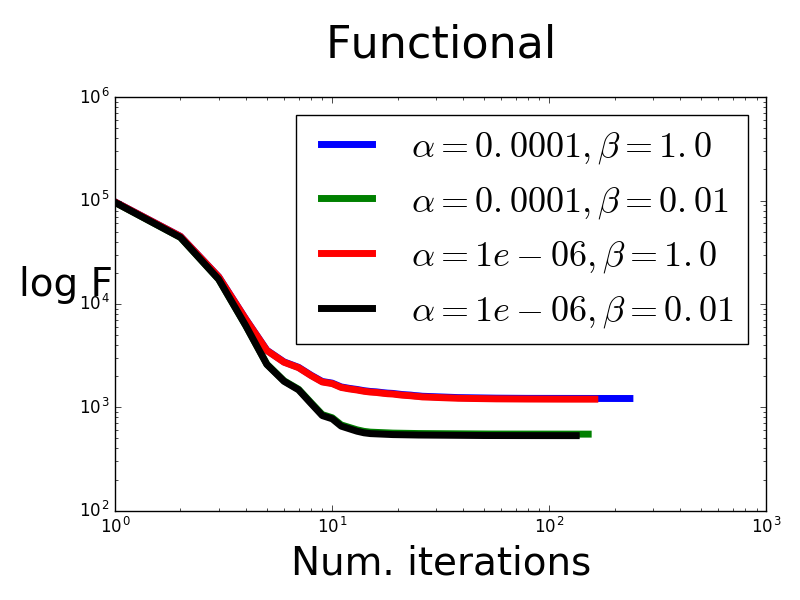
\includegraphics[scale=0.2]{Convergence0}  
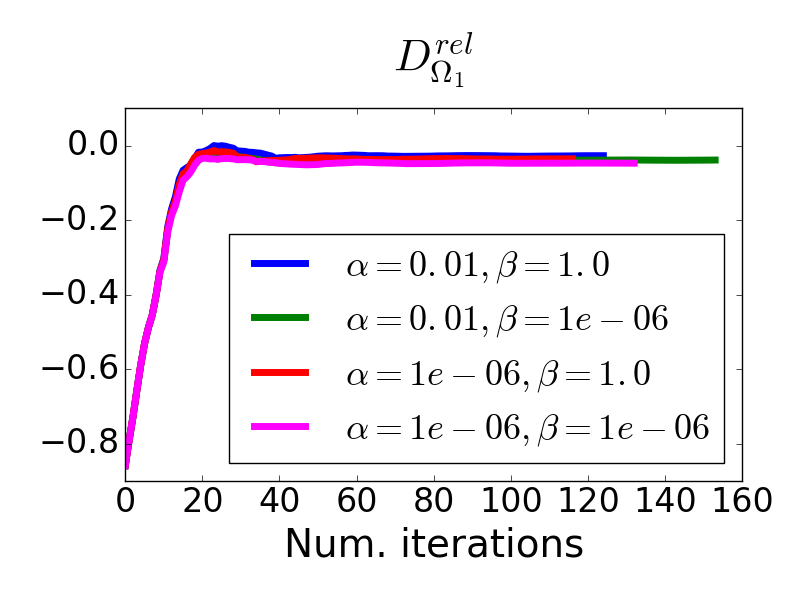
\includegraphics[scale=0.2]{Convergence1}  
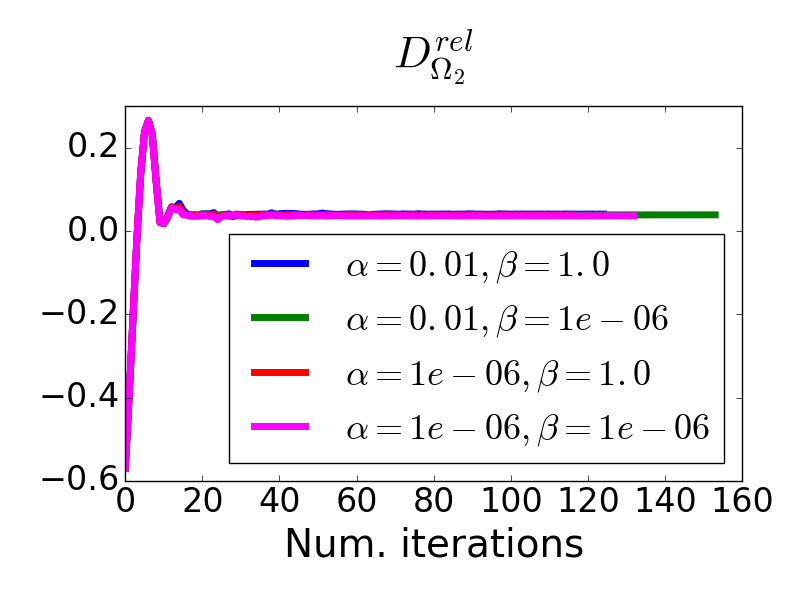
\includegraphics[scale=0.2]{Convergence2}  
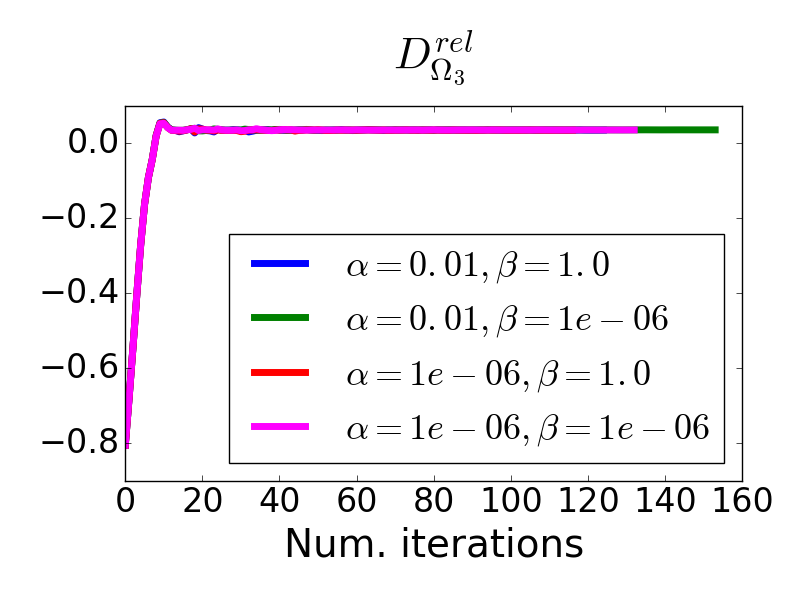
\includegraphics[scale=0.2]{Convergence3}  
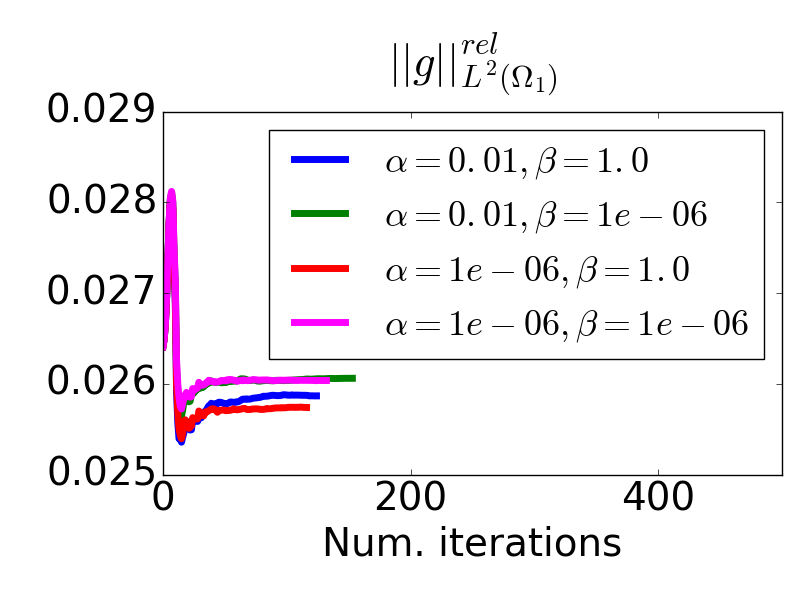
\includegraphics[scale=0.2]{Convergence4}  
\label{convergence}
\caption{Convergence of the diffusion coefficients, boundary conditions and functional with respect to different $\alpha$ and $\beta$ values. } 
\label{convergence}
\end{figure}

\subsubsection{The number of timessteps}
Increasing the number of time-steps in the computations can potentially allow for a more accurate temporal reconstruction, but at the same time the number of observations per control decreases and the regularization may therefore play a larger role. Furthermore, the computational cost will rise with additional time-steps. Thus finding the optimal number of time-steps can be essential for larger problems. The computation varied the regularization parameters with 20 and 40 timesteps.

The results are given in Tab.\ref{TAB::timesteps}, and it can be seen for all $\alpha=1.0$ that the relative error becomes bigger with more time-steps. This behavior can also be seen for $\alpha=1.0e-2$ and $\beta < 1.0e-2$, which implies an interaction between the regularization parameters. 
Therefore $g$ was investigated by plotting boundary points through time for different values of $\alpha$ and $\beta$, see Fig \ref{boundarycontrol}. In Figure \ref{boundarycontrol} we can see that more time-steps causes  oscillations for $\alpha=1.0$, and each peak corresponds to a observation time. These oscillations are caused by $\alpha$, which tries minimize $g$ between observation times.

It can be seen that more time-steps causes an increase number of iterations, but for some values the number of iterations decreases. These values share that $\alpha $ is a magnitude 2 lower than $ \beta$,i.e $\alpha=1.0e-2$ and $\beta =1.0$. This indicates that $\alpha $ should be smaller than $\beta$ to achieve optimal convergence. However, the number of iterations in Table ~\ref{Tab::1} are smaller for all regularization parameters. 


\subsubsection{The number of observations}
The dependency on observations is relevant, since the number of observations of the MRI data is limited. This was investigated by changing the number of observations, and examine the results. The number of observation were chosen to be 5 and 20, and the observation times were evenly spaced. 


The results are shown in Tab.\ref{TAB::double} and Tab.\ref{TAB::half}. In Tab.\ref{TAB::half}, the values $\alpha =1.0e-2$ and $\beta<1.0$ gives a surge in the relative error with more time-steps. This behavior is neither visible in Tab.\ref{TAB::timesteps} or Tab.\ref{TAB::double} given the same regularization parameters. It seems likely that this error is caused by oscillations, seen in Figure~\ref{boundarycontrol}.  

The observations acts as stabilization for the functional, which gives a broader range of adequate regularization parameters.

%In Table ~\ref{TAB::double}, we can see that $\aplha < 1.0e-2$ and $\beta =1.0e-2$ have a drastic change in the number of iteration for $20$ time-steps. 




\begin{figure}
\centering
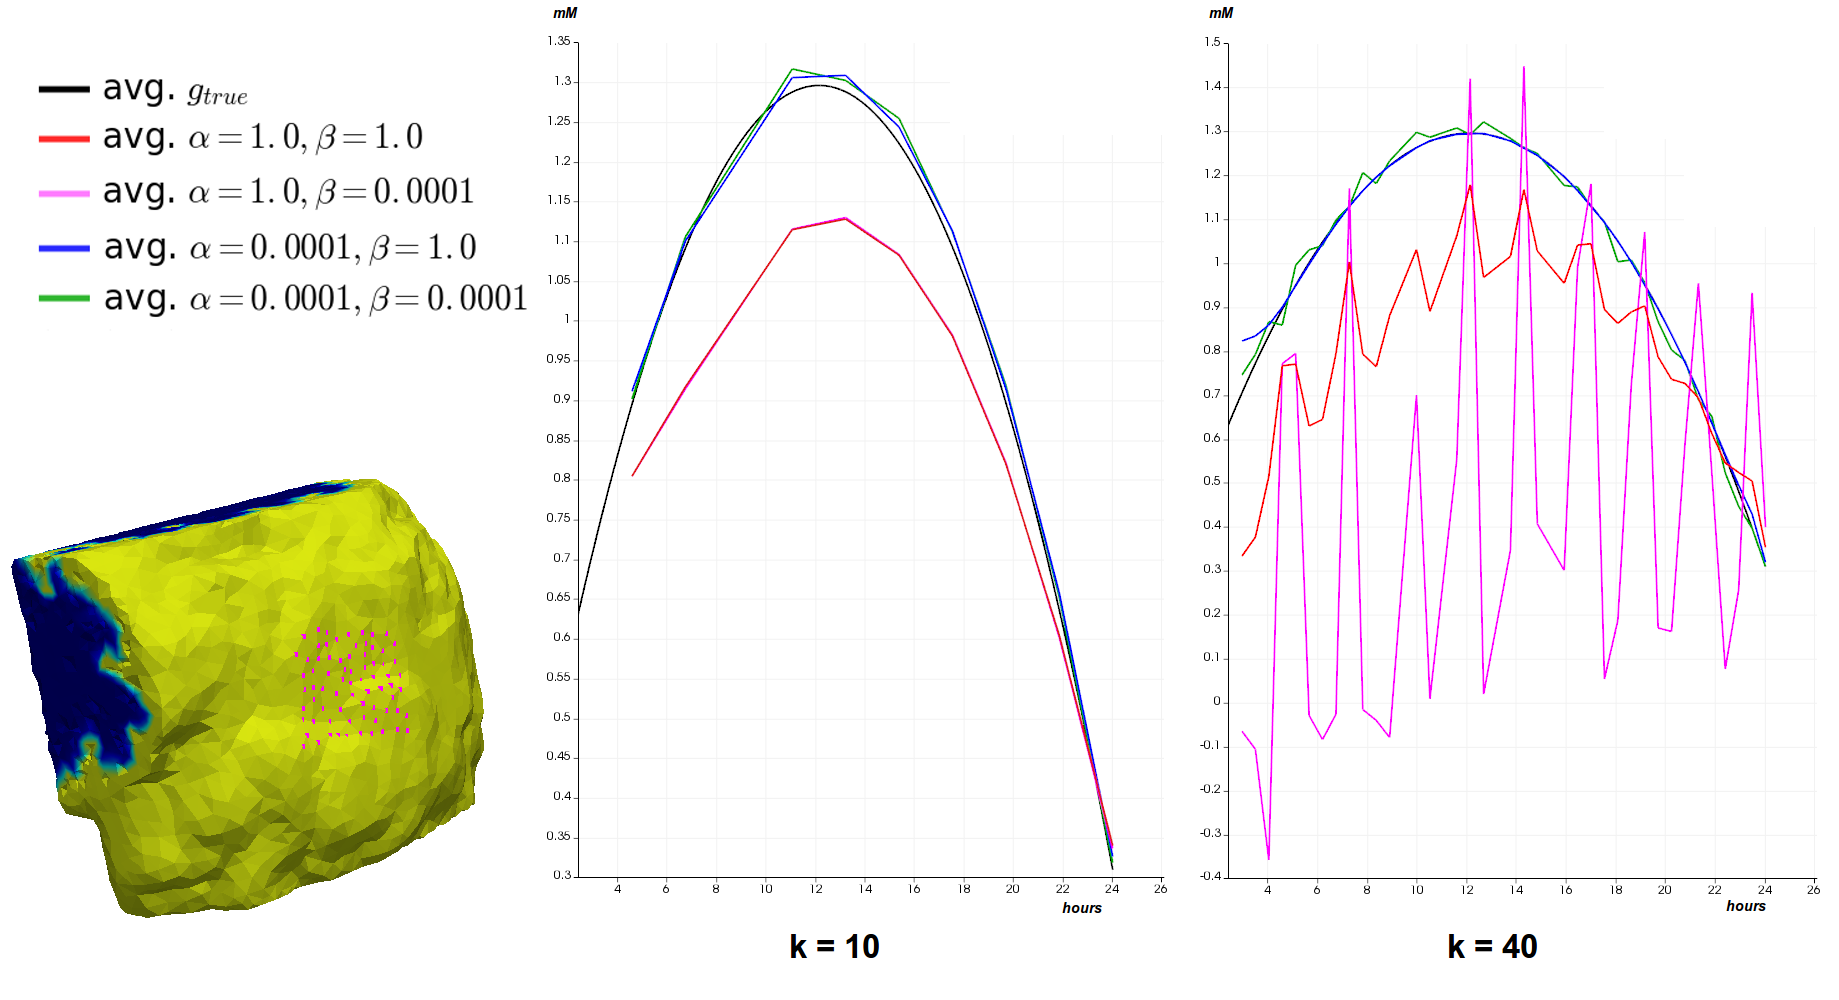
\includegraphics[scale=0.2]{boundary_control.png}  
\caption{ Displays plots over time for a selection of points at the boundary of $\Omega_1$ with different regularization parameters and number of timesteps $k$. The left panel shows the legend for the plot over time, together with the selection of points. The middle panel shows the average boundary value $g$ for different regularization parameter with $k=10$. The right panel shows the average boundary value $g$ for different regularization parameter with $k=40$. }
\label{boundarycontrol}
\end{figure}

\subsubsection{The noise susceptibility}
The MRI data contains noise, hence an investigation to the noise susceptibility is needed. This was done by adding uniform noise in the range $\lbrace -n_{amp} , n_{amp} \rbrace $, with $n_{amp}$ defined as noise amplitude, to the manufactured observations. Then the optimization was solved by varying the regularization parameters $\alpha$ and $\beta$. Figure~\ref{12hourswithnoise} and Figure~\ref{24hourswithnoise} show the reconstruction of the manufactured solution with 
different noise levels with $\alpha=0.0001$ and $\beta=1.0$. Clearly, the reconstruction shown in the lower rows is quite robust with respect to the various levels
of noise shown in the upper rows.      

In Tabel~\ref{Tab::Noise0.03}, we can see that a noise amplitude of 0.03, (10$\%$ of maximum initial condition) had negligible effect on the relative error. However, in Tabel~\ref{Tab::Noise0.3} the noise amplitude was increased to 0.3 (100$\%$ of maximum initial condition) and it is observed that for  $\alpha \leq 1.0e-4$  and $\beta \leq 1.0e-4$ the optimization failed to converge before reaching maximum iteration of 1000 steps. Furthermore, the relative boundary error $||g||\sp{rel}_{L\sp{2}(\Omega_1)}$ is larger for lower values of $\beta$.  




\begin{figure}
\centering
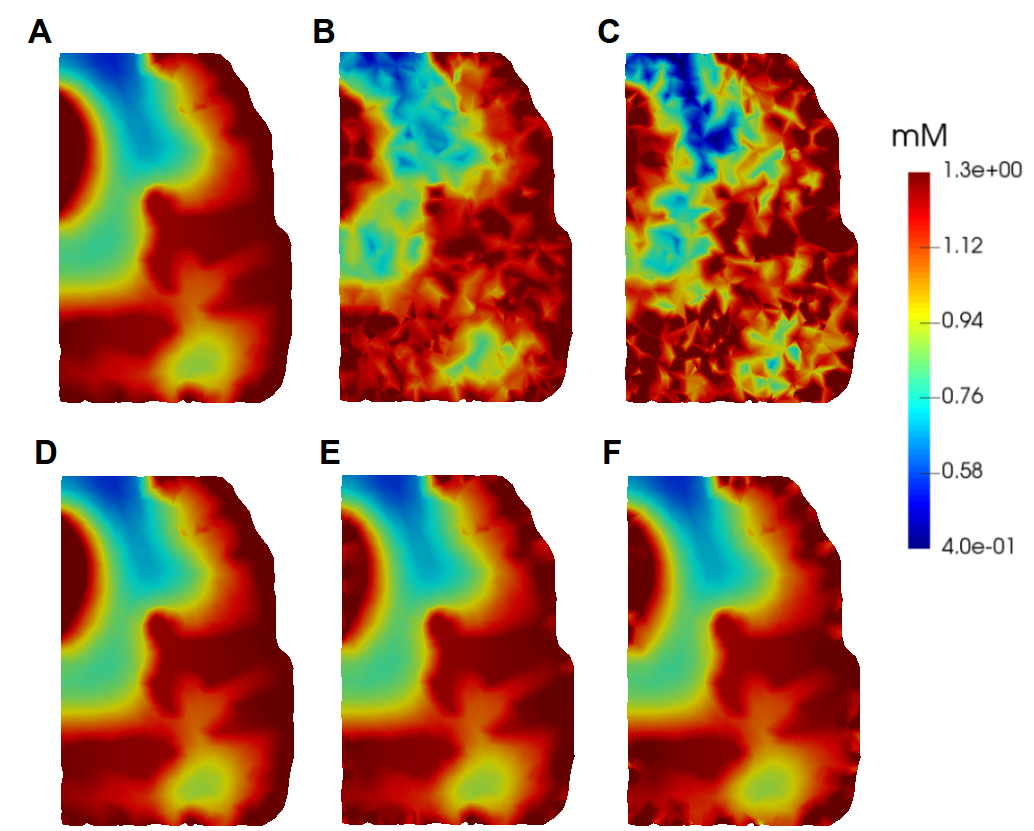
\includegraphics[scale=0.4]{noise-12.png}  
\caption{The upper row shows the manufactured observation, A ) Shows the manufactured observation at time-point 24 with no noise added. B) Shows the manufactured observation at time-point 24 with an noise amplitude of 0.15. C)Shows the manufactures observation at time-point 24 with noise amplitude of 0.3. The lower row shows the results with optimized parameter obtained with $\alpha=0.0001$, $\beta=1.0$ and $k=27$. D) Shows the resulting state given the observation in A. E)  Shows the resulting state given the observation in B .F) Shows the resulting state given the observation in C. }
\label{12hourswithnoise}
\end{figure}


\begin{figure}
\centering
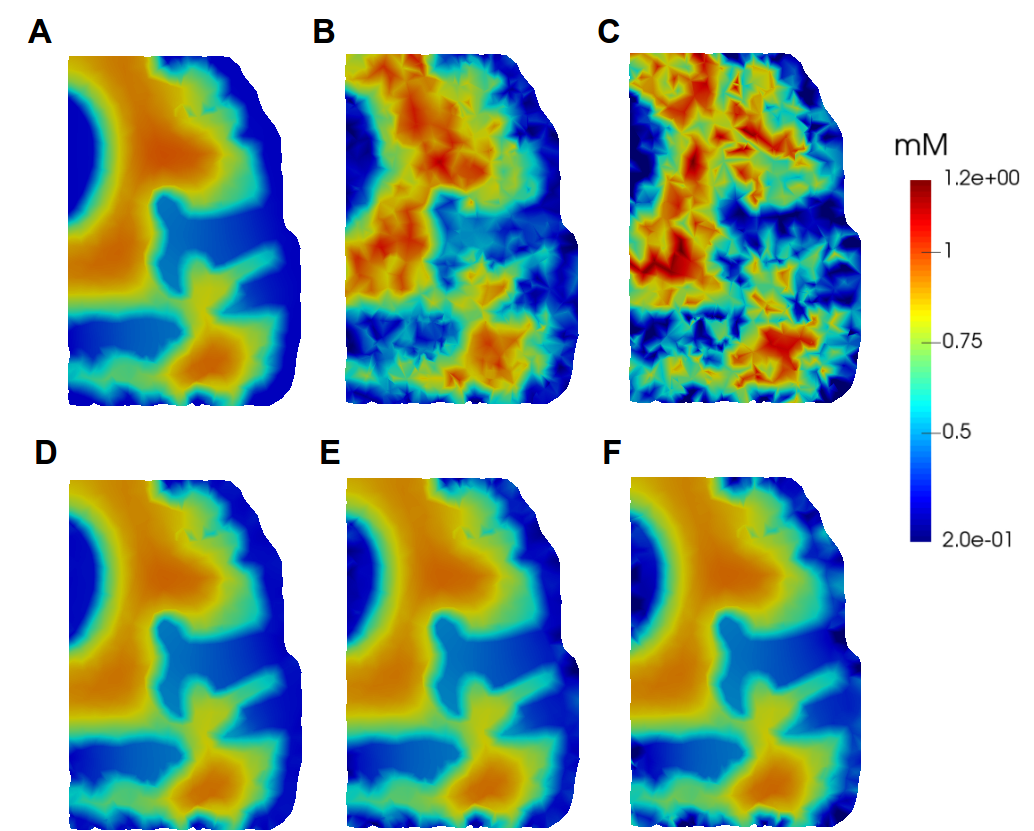
\includegraphics[scale=0.4]{noise-24.png}
\caption{The upper row shows the manufactured observation, A ) Shows the manufactured observation at time-point 24 with no noise added. B) Shows the manufactured observation at time-point 24 with a noise amplitude of 0.15. C)Shows the manufactures observation at time-point 24 with noise amplitude of 0.3. The lower row shows the results with optimized parameter obtained with $\alpha=0.0001$, $\beta=1.0$ and $k=20$. D) Shows the resulting state given the observation in A. E)  Shows the resulting state given the observation in B .F) Shows the resulting state given the observation in C.  }
\label{24hourswithnoise}
\end{figure}




%\subsection{Sparse observations}
%The MRI data contains observations after the injection of CSF tracer. These observation are unevenly distributed in time resulting in large time intervals with no observations. Therefore the effect of these temporal gaps in the observations will be evaluated. This was done by selecting the observation times as follows  $t_i = \lbrace$0.8, 1.0, 1.2, 1.8, 2.4, 3.6, 5.4, 7.6, 24.0$\rbrace$. The regularization parameters was selected, so that the error would be minimized,and noise was also added.
%
%The results are shown in Tab.\ref{Tab::Hole1} and Tab\ref{Tab::Hole2}, and it can be observed that the addition of noise caused $\beta=1.0$ to converge the same. Comparing the values in Tab\ref{Tab::Hole1} and Tab.\ref{TAB::timesteps}, showed that the relative error increased.  

\subsection{A Real case} 

\subsubsection{Results obtained when using real observations}
The MRI data consisted of the observations at times $t_i \in \lbrace$ 0.00, 0.16, 0.39, 0.55, 0.77, 2.09, 6.05, 24., 48., 698. $\rbrace (hours)$ with the time $t_i=0.00$ as the observation 1-2 hours after the tracer was injected. There was no significant visible change in the tracer between the observations at $\lbrace $ 0.00, 0.16, 0.39, 0.55, 0.77 $ \rbrace$. This prompted the use of the following observation times  $0.00, 2.09, 6.05, 24., 48.$. 

The estimation of tracer concentration proved difficult in the CSF compartment. Therefore the 2 domain mesh, shown in Fig.\ref{Fig::Mesh} was used in the computation. The boundary control was set to the external boundary of both domains, and the subscript in $D_w$ and $D_g$ denotes white and grey diffusion coefficients. Furthermore, bounds were added to the L-BFGS-B algorithm to ensure non-negative boundary controls and the convergence criteria was adjusted to $\epsilon=6.0e-1$. The number of timesteps were selected to be $k=24$ and $k=48$, which gives $dt = 2 hour$ and $dt = 1 hour$.   

The results are shown in Tab.\ref{Tab::Real-data}, and the observations after 12 and 48 hours were compared with the corresponding states in Figure~\ref{Fig::realdata}. From Table~\ref{Tab::Real-data},it can be observed that $D_w$ have a higher value for $\alpha =1.0e-2$.

\subsubsection{Comparison with results obtained from DTI analysis}

The median diffusion coefficient in the DTI was estimated to be $8.7e-4 \mathrm{mm\sp{2}/s}$ in white matter and $1.0e-3 \mathrm{mm\sp{2}/s}$ in grey matter. This corresponds to a tortuosity of $1.85$ and $1.73$, given that the self-diffusivity of water has been estimated to be around $3.0e-3\mathrm{mm\sp{2}/s}$ at $37\sp{o}C$. Fhe reference value $3.8e-4 \mathrm{mm\sp{2}/s}$ for Gd-DPTA gives an estimate for the apparent diffusion coefficient in the grey and white matter to respectively be $ 1.26e-4\mathrm{mm\sp{2}/s}$ and $1.10e-4 \mathrm{mm\sp{2}/s}$. This estimation assumes that the tortuosity is independent on molecular size. 

The oscillation in Fig.\ref{boundarycontrol} showed a large discrepancy in the states between observations. Therefore the states with $k=48$ were examined after 36 hours, see Figure\ref{statecomparison}. It can be observed that the upper right row displays a discrepancy, which likely due to inadequate regularization parameters. Furthermore, we can see that for $\alpha=1.0e-2$ there is a clear discrepancy in the diffusion coefficients compared to other values $\alpha$. This prompt the exclusion of the corresponding values, which gives an average computed values $ 0.65 \mathrm{mm\sp{2}/h}$ and  $ 0.8 \mathrm{mm\sp{2}/h}$ in respectively grey and white matter. Scaled to $\mathrm{mm\sp{2}/s}$ gives the corresponding values $1.8e-4\mathrm{mm\sp{2}/s}$ and $2.22e-4 \mathrm{mm\sp{2}/s}$. 

\subsection*{Compare high DTI values with computed}
This gives a difference of $42 \%$ in grey matter and $ 100 \%$ in white matter compared to the estimated values using DTI.

In Fig.\ref{Fig::realdata}, it can be seen that there were regions with negligible amount of tracers and vice versa. The regions with above average amount of tracers corresponds with high diffusivity regions in Figure~\ref{figuredti}. This suggests that the computed diffusion coefficients corresponds to these values. The ADC value in the high diffusivity regions are closer to  $1.4e-3 \mathrm{mm\sp{2}/s}$, which corresponds to estimated diffusion coefficient of value $1.5e-3 \mathrm{mm\sp{2}/s}$. This gives a difference of $ 46 \%$ compared to the computed values. 


















%The region with high diffusivity in the white matter, shown in Fig\ref{FIG::DTI}, gives a upper bound on the diffusion coefficient to be 1.3 $\mathrm{mm\sp{2}/s}$. 



%
% \begin{table}
%\centering
%\caption{Viser omgjøringer,estiamering og prosentvis forskjell for min og max control/optimerte verdier . Unit $\left[ \mathrm{mm\sp{2}/h} \right]$}
%\resizebox{\textwidth}{!}{\begin{tabular}{*{6}c}
%$ D\sp{free}_{water} $ & $ D\sp{DTI}__{g} $ & $ D\sp{DTI}_{w} $ & $D\sp{fre}__{Gd-DPTA} $ & $D\sp{ADC}__{g} $ & $ D\sp{ADC}_{w} $ & $ D\sp{ADC}_{g} -D\sp{OPT}_{g} $ &$ D\sp{ADC}_{w} -D\sp{OPT}_{w} $ \\
%\hline
%10.8 & 3.64 & 3.13 & 1.37 & 0.46 & 0.40 &  20 - 114 $\%$  & 100- 200 $\%$
%  -   &  -    & 4.86 &  - &  -   & 0.61 &   -                  &   0 - 100 $\%$       
%\end{tabular}} 
%\label{}
%\end{table} 
% 
%The region with high diffusivity in the white matter, shown in Fig\ref{FIG::DTI}, gives a upper bound on the diffusion coefficient to be 1.3 $\mathrm{mm\sp{2}/s}$

\section{Discussion}

The methodology presented here for identification of diffusion coefficients and boundary conditions with application to the glymphatic system appears to work quite 
well for regularization parameters varying by orders of magnitude. It is particularly interesting to see that the procedure efficiently removes noise as demonstrated
in the Figures \ref{12hourswithnoise} and \ref{24hourswithnoise} with noise levels of 30\% \kam{is this correctly stated}{\color{red} (0.3,-0.3) added to all values in range (0,g(t))}. 
Crucial in our application is the interplay between the regularization term that regulates the smoothness of the boundary conditions as well as
the integrate magnitude of the boundary conditions over time, i.e. $\alpha$ and $\beta$, and the
importance of interplay of these parameter increases with the number of time steps. This is, however, not surprising because our observations are sparse
in time and hence an oscillating boundary condition in time will minimized the integrated boundary condition at the cost of reducing the smoothness in time.         

While a more comprehensive study involving more patients would be required in order to assess whether the clearance here happens faster than diffusion (\kam{egentlig er
vel dette det motsatte av clearance} a few remarks are in order. We find that the diffusion coefficients is XXX larger than what was found by the DTI modality.  
However, we have not yet been able to assessment the self-diffusion of water as well as the diffusivity of Gadovist used in this study in phantom models. As such 
the constants in equation XXX must be taken with caution. Furthermore,    
the computational model assumes isotropic diffusivity, but the anisotropy in the white matter is well documented, as shown by the FA in Fig\ref{figuredti}. It can be seen in Figure~\ref{Fig::realdata} that the region with high FA have negligible amounts of tracer present. Therefore it would seem that the anisotropy do not have direct impact on the computations, since the computation can not evaluate a static environment. Therefore  observation of tracer in regions with anisotropy can be considered a requirement for adding anisotropy to the model.
The regions with high diffusivity in Figure~\ref{figuredti},  have significant amount of diffusivity as seen in Figure~\ref{Fig::realdata} 


The computational model have 2 global controls for the diffusion coefficients, while it can be seen in  Fig.\ref{figuredti} that diffusion coefficients can be considered a spacial function. The implementation control parameters for each dofs would significantly increase the computational cost. The option using region specific control parameters seems to be a better option, since the diffusivity appears to be regional. It can also be taken into consideration to model the diffusion coefficients as a function in time, given the report of an increase clearance in rodents during sleeping \cite{xie2013sleep}. This would indicate a time-dependent diffusivity, since the clearance in the brain is driven by diffusion. The time-dependency would correspond to a change in tortuosity, since properties of the tracer molecule do not change.

In Tab.\ref{Tab::Real-data}, it is shown that the grey matter diffusion coefficient have a consistent increase based on the decrease in the relaxation parameter $\beta$. This can be caused by the boundary control $g$, which exists along the entire boundary of the grey matter. Considering the that the grey matter volume has a depth less than 3 mm makes it susceptible to changes in $g$. This can be observed in the reconstruction in Fig.\ref{12hourswithnoise} and Fig.\ref{24hourswithnoise}, where the noise is present at the boundary.
  

The hypothesis of the glymphatic system \cite{iliff2012paravascular} states that the waste is cleared through the veins in the parenchyma. This gives the tracer additional pathways that is not considered in the computational model. These additional pathways can be modeled as a drainage, which can be included as a control source term. 



 
\section{Conclusion}

It can be concluded from the results that increasing the number of iterations gives rise to oscillations for poor regularizations parameters. 


%\begin{figure}
%\centering
%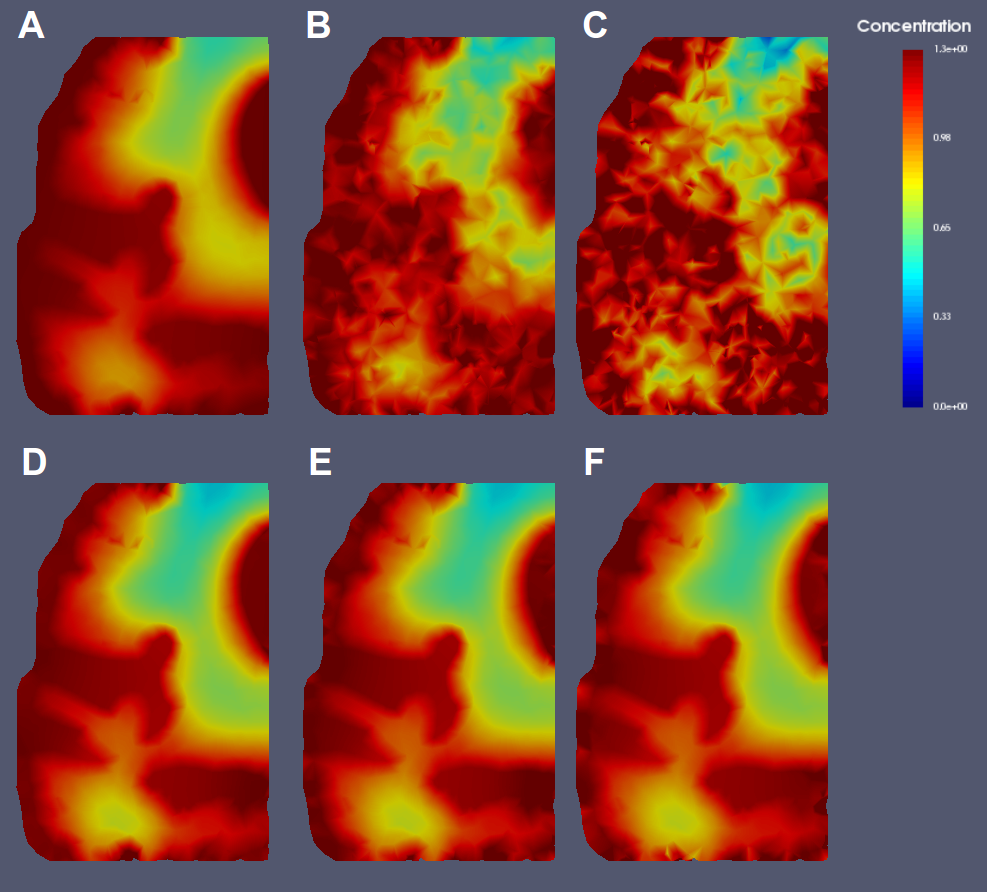
\includegraphics[scale=0.4]{27-12-hours-scale-0-1-3.png}  
%\caption{The upper row shows the manufactured observation, A ) Shows the manufactured observation at time-point 24 with no noise added. B) Shows the manufactured observation at time-point 24 with an noise amplitude of 0.15. C)Shows the manufactures observation at time-point 24 with noise amplitude of 0.3. The lower row shows the results with optimized parameter obtained with $alpha=0.0001$, $\beta=1.0$ and $k=27$. D) Shows the resulting state given the observation in A. E)  Shows the resulting state given the observation in B .F) Shows the resulting state given the observation in C. }
%\end{figure}
%
%
%\begin{figure}
%\centering
%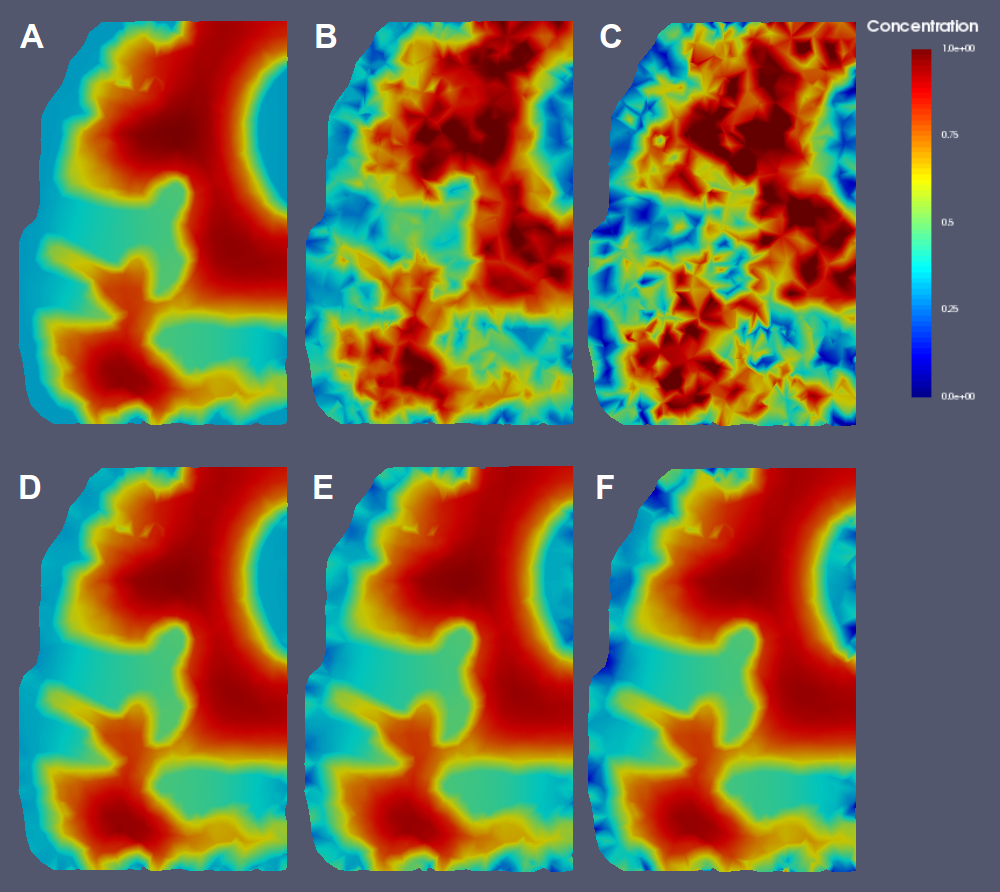
\includegraphics[scale=0.4]{27-24-hours-scale-0-1.png}
%\caption{The upper row shows the manufactured observation, A ) Shows the manufactured observation at time-point 24 with no noise added. B) Shows the manufactured observation at time-point 24 with a noise amplitude of 0.15 {\color{red} explain noise ampliutde}. C)Shows the manufactures observation at time-point 24 with noise amplitude of 0.3. The lower row shows the results with optimized parameter obtained with $alpha=0.0001$, $\beta=1.0$ and $k=27$. D) Shows the resulting state given the observation in A. E)  Shows the resulting state given the observation in B .F) Shows the resulting state given the observation in C.  }
%\end{figure}
% 
% 
% 
%
% 
\section{References}


\bibliographystyle{amsplain}
\bibliography{references}

 



 
\begin{figure}
\centering
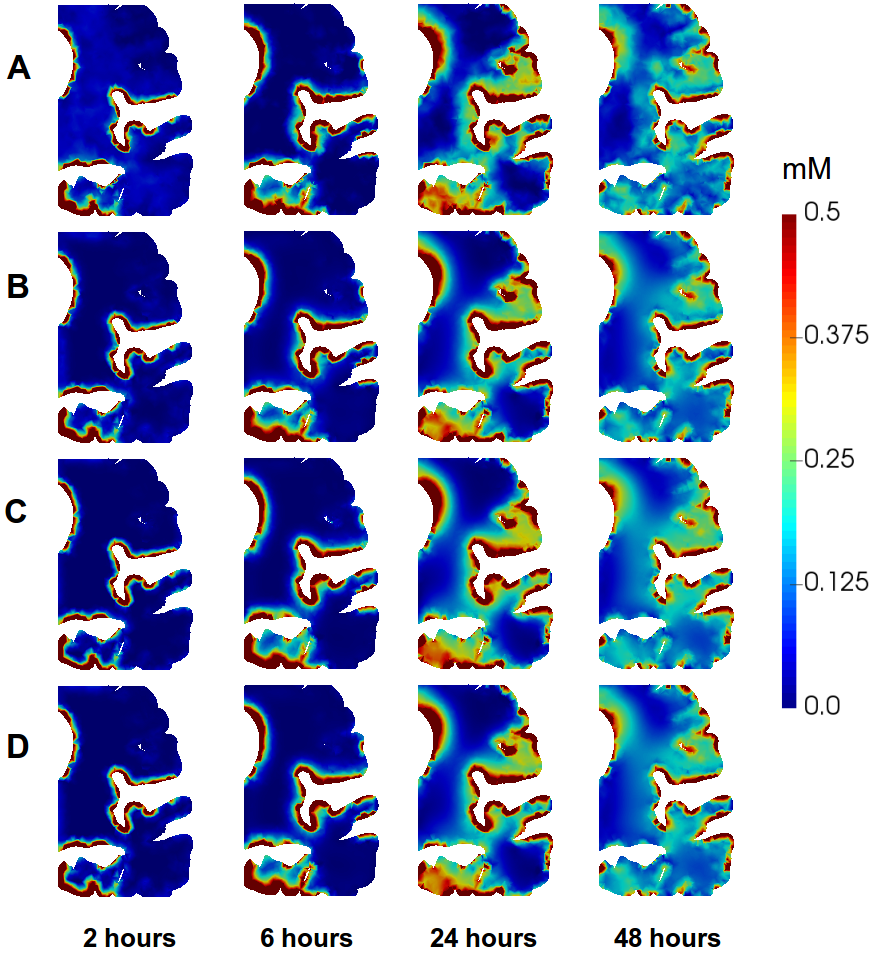
\includegraphics[width=0.95\textwidth]{different.png} 
\caption{Row A) shows the observation at times 2 hours, 6 hours, 24 hours and 48 hours after the first observation with tracer. Row B) shows the corresponding states with the relaxation parameters $\alpha=0.01$ and $\beta=0.01$ and $k=48$.   Row C) shows the corresponding states with the relaxation parameters $\alpha=0.0001$ and $\beta=1.0$ and $k=48$
 Row D) shows the corresponding states with the relaxation parameters $\alpha=1.0e-6$ and $\beta=0.1$ and $k=48$. The color-bar was restricted to the range $ \lbrace 0 ,0.5 \rbrace$. }
\label{Fig::realdata}
\end{figure}

\begin{figure}
\centering
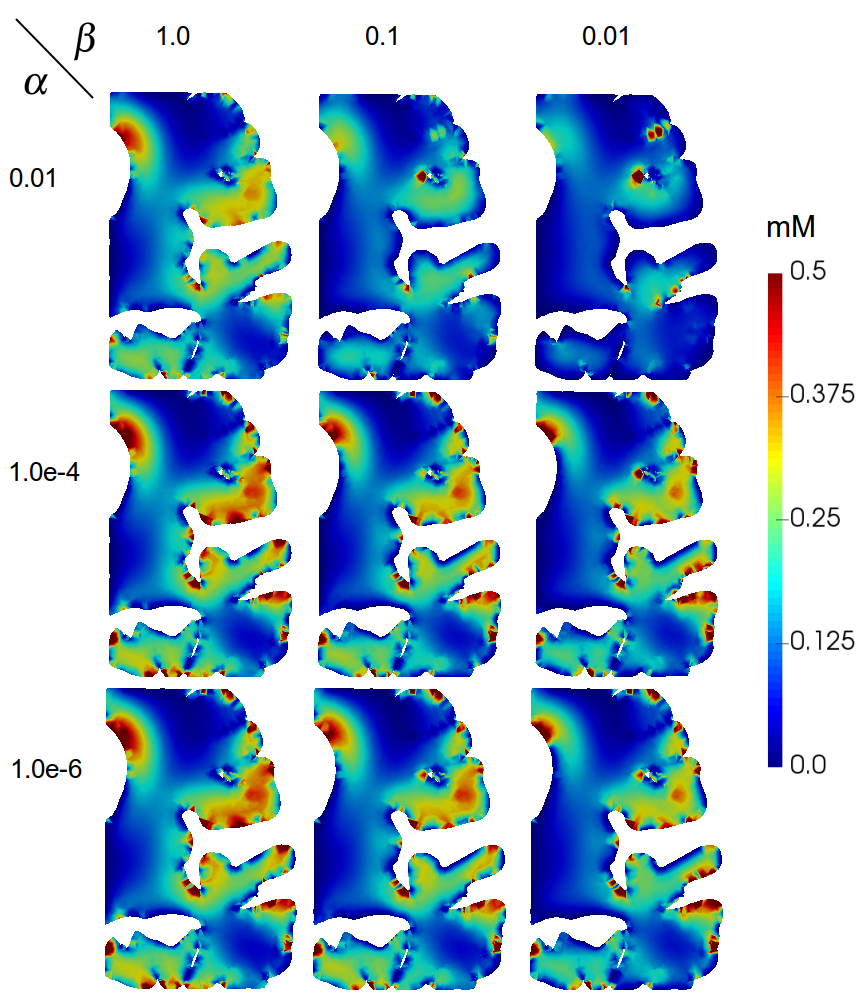
\includegraphics[width=0.95\textwidth]{Statecomparison36h-pinta.png} 
\caption{ Displays the states for different regularization parameters after 36 hours for $k=48$.}
\label{statecomparison}
\end{figure}

 


\begin{table}
\centering
\caption{Shows the regularization parameters $\alpha$ and $\beta$, number of timesteps $k$ and number of observation $\tau$ with the resulting number of iterations and the relative error for the control parameters. {\color{red} check pvd }.}
\begin{tabular}{*{8}c}
$\alpha$ & $\beta$ & k  & iter & $ D_{\Omega_1}\sp{rel}$ & $ D_{\Omega_2}\sp{rel} $ & $D_{\Omega_3}\sp{rel}$ & $||g||_{rel}$ \\
\hline 
 1.0e+00 	 & 1.0e+02 	 & 10 & 437 	 & +4.631 & +0.283 & +0.103 & +0.127 \\ 
 1.0e+00 	 & 1.0e+00 	 & 10 & 129 	 & +1.638 & +0.224 & +0.089 & +0.119 \\ 
 1.0e+00 	 & 1.0e-02 	 & 10 & 129 	 & +1.602 & +0.223 & +0.089 & +0.119 \\ 
 1.0e+00 	 & 1.0e-04 	 & 10 & 151 	 & +1.608 & +0.223 & +0.089 & +0.119 \\ 
 1.0e+00 	 & 1.0e-06 	 & 10 & 133 	 & +1.603 & +0.223 & +0.089 & +0.119 \\ 
 1.0e-02 	 & 1.0e+02 	 & 10 & 186 	 & +0.649 & +0.111 & +0.036 & +0.033 \\ 
 1.0e-02 	 & 1.0e+00 	 & 10 & 125 	 & -0.027 & +0.041 & +0.036 & +0.026 \\ 
 1.0e-02 	 & 1.0e-02 	 & 10 & 133 	 & -0.039 & +0.039 & +0.036 & +0.026 \\ 
 1.0e-02 	 & 1.0e-04 	 & 10 & 108 	 & -0.039 & +0.039 & +0.036 & +0.026 \\ 
 1.0e-02 	 & 1.0e-06 	 & 10 & 154 	 & -0.039 & +0.039 & +0.036 & +0.026 \\ 
 1.0e-04 	 & 1.0e+02 	 & 10 & 212 	 & +0.636 & +0.108 & +0.035 & +0.032 \\ 
 1.0e-04 	 & 1.0e+00 	 & 10 & 143 	 & -0.036 & +0.039 & +0.035 & +0.026 \\ 
 1.0e-04 	 & 1.0e-02 	 & 10 & 108 	 & -0.047 & +0.037 & +0.036 & +0.026 \\ 
 1.0e-04 	 & 1.0e-04 	 & 10 & 158 	 & -0.047 & +0.037 & +0.036 & +0.026 \\ 
 1.0e-04 	 & 1.0e-06 	 & 10 & 142 	 & -0.047 & +0.037 & +0.036 & +0.026 \\ 
 1.0e-06 	 & 1.0e+02 	 & 10 & 203 	 & +0.636 & +0.108 & +0.035 & +0.032 \\ 
 1.0e-06 	 & 1.0e+00 	 & 10 & 117 	 & -0.035 & +0.039 & +0.035 & +0.026 \\ 
 1.0e-06 	 & 1.0e-02 	 & 10 & 120 	 & -0.047 & +0.037 & +0.036 & +0.026 \\ 
 1.0e-06 	 & 1.0e-04 	 & 10 & 122 	 & -0.047 & +0.037 & +0.036 & +0.026 \\ 
 1.0e-06 	 & 1.0e-06 	 & 10 & 133 	 & -0.047 & +0.037 & +0.036 & +0.026 \\ 
%  1.0e+00 	 & 1.0e+02 	 & 10 & 499 	 & +5.125 & +0.278 & +0.105 & +0.127 \\ 
%  1.0e+00 	 & 1.0e+00 	 & 10 & 225 	 & +4.148 & +0.304 & +0.092 & +0.135 \\ 
%%\rowcolor{red}  1.0e+00 	 & 1.0e-01 	 & 10 & 206 	 & +4.272 & +0.305 & +0.091 & +0.142 \\ 
% 1.0e+00 	 & 1.0e-02 	 & 10 & 233 	 & +4.272 & +0.305 & +0.091 & +0.143 \\ 
%%\rowcolor{red}  1.0e+00 	 & 1.0e-03 	 & 10 & 208 	 & +4.437 & +0.305 & +0.091 & +0.143 \\ 
% 1.0e+00 	 & 1.0e-04 	 & 10 & 204 	 & +4.271 & +0.306 & +0.091 & +0.143 \\ 
%%\rowcolor{red}  1.0e+00 	 & 1.0e-05 	 & 10 & 203 	 & +4.400 & +0.305 & +0.091 & +0.143 \\ 
% 1.0e+00 	 & 1.0e-06 	 & 10 & 222 	 & +4.584 & +0.304 & +0.090 & +0.143 \\
% 
%% 1.0e-01 	 & 1.0e+00 	 & 10 & 207 	 & +0.127 & +0.093 & +0.041 & +0.027 \\ 
% %1.0e-01 	 & 1.0e-01 	 & 10 & 196 	 & +0.121 & +0.093 & +0.041 & +0.046 \\ 
%% 1.0e-01 	 & 1.0e-02 	 & 10 & 232 	 & +0.123 & +0.093 & +0.041 & +0.056 \\ 
% %1.0e-01 	 & 1.0e-03 	 & 10 & 183 	 & +0.122 & +0.093 & +0.040 & +0.057 \\ 
%% 1.0e-01 	 & 1.0e-04 	 & 10 & 212 	 & +0.122 & +0.093 & +0.040 & +0.057 \\ 
% %1.0e-01 	 & 1.0e-05 	 & 10 & 168 	 & +0.122 & +0.093 & +0.041 & +0.057 \\
%% 1.0e-01 	 & 1.0e-06 	 & 10 & 195 	 & +0.122 & +0.093 & +0.041 & +0.057 \\ 
% 1.0e-02 	 & 1.0e+02 	 & 10 & 228 	 & +0.702 & +0.106 & +0.035 & +0.033 \\ 
% 1.0e-02 	 & 1.0e+00 	 & 10 & 227 	 & +0.015 & +0.067 & +0.039 & +0.018 \\ 
% %1.0e-02 	 & 1.0e-01 	 & 10 & 153 	 & +0.006 & +0.065 & +0.039 & +0.021 \\ 
% 1.0e-02 	 & 1.0e-02 	 & 10 & 184 	 & +0.005 & +0.065 & +0.039 & +0.039 \\ 
% %1.0e-02 	 & 1.0e-03 	 & 10 & 176 	 & +0.004 & +0.065 & +0.039 & +0.048 \\ 
% 1.0e-02 	 & 1.0e-04 	 & 10 & 195 	 & +0.005 & +0.065 & +0.039 & +0.049 \\ 
% %1.0e-02 	 & 1.0e-05 	 & 10 & 215 	 & +0.004 & +0.065 & +0.039 & +0.051 \\ 
% 1.0e-02 	 & 1.0e-06 	 & 10 & 205 	 & +0.005 & +0.065 & +0.039 & +0.050 \\ 
%
% %1.0e-03 	 & 1.0e+00 	 & 10 & 179 	 & +0.004 & +0.064 & +0.039 & +0.019 \\ 
% %1.0e-03 	 & 1.0e-01 	 & 10 & 221 	 & -0.005 & +0.063 & +0.039 & +0.018 \\ 
% %1.0e-03 	 & 1.0e-02 	 & 10 & 89 	 & -0.007 & +0.063 & +0.039 & +0.026 \\ 
% %1.0e-03 	 & 1.0e-03 	 & 10 & 77 	 & -0.005 & +0.062 & +0.039 & +0.027 \\ 
% %1.0e-03 	 & 1.0e-04 	 & 10 & 100 	 & -0.006 & +0.062 & +0.039 & +0.027 \\ 
% %1.0e-03 	 & 1.0e-05 	 & 10 & 105 	 & -0.006 & +0.062 & +0.039 & +0.027 \\ 
% %1.0e-03 	 & 1.0e-06 	 & 10 & 123 	 & -0.007 & +0.062 & +0.039 & +0.028 \\ 
%
% 1.0e-04 	 & 1.0e+02 	 & 10 & 167 	 & +0.688 & +0.104 & +0.035 & +0.032 \\ 
% 1.0e-04 	 & 1.0e+00 	 & 10 & 236 	 & +0.004 & +0.063 & +0.039 & +0.019 \\ 
% %1.0e-04 	 & 1.0e-01 	 & 10 & 195 	 & -0.006 & +0.062 & +0.039 & +0.018 \\ 
% 1.0e-04 	 & 1.0e-02 	 & 10 & 152 	 & -0.006 & +0.062 & +0.039 & +0.022 \\ 
% %1.0e-04 	 & 1.0e-03 	 & 10 & 119 	 & -0.008 & +0.062 & +0.039 & +0.026 \\ 
% 1.0e-04 	 & 1.0e-04 	 & 10 & 106 	 & -0.007 & +0.062 & +0.039 & +0.026 \\ 
% %1.0e-04 	 & 1.0e-05 	 & 10 & 109 	 & -0.007 & +0.062 & +0.039 & +0.026 \\ 
% 1.0e-04 	 & 1.0e-06 	 & 10 & 99 	 & -0.008 & +0.062 & +0.039 & +0.026 \\
% 
% %1.0e-05 	 & 1.0e+00 	 & 10 & 139 	 & +0.004 & +0.063 & +0.039 & +0.019 \\ 
% %1.0e-05 	 & 1.0e-01 	 & 10 & 170 	 & -0.006 & +0.062 & +0.039 & +0.018 \\ 
% %1.0e-05 	 & 1.0e-02 	 & 10 & 182 	 & -0.007 & +0.062 & +0.039 & +0.020 \\ 
% %1.0e-05 	 & 1.0e-03 	 & 10 & 70 	 & -0.007 & +0.062 & +0.039 & +0.026 \\ 
% %1.0e-05 	 & 1.0e-04 	 & 10 & 77 	 & -0.007 & +0.062 & +0.039 & +0.026 \\ 
% %1.0e-05 	 & 1.0e-05 	 & 10 & 104 	 & -0.008 & +0.062 & +0.039 & +0.026 \\ 
% %1.0e-05 	 & 1.0e-06 	 & 10 & 92 	 & -0.007 & +0.062 & +0.039 & +0.026 \\ 
% 1.0e-06 	 & 1.0e+02 	 & 10 & 210 	 & +0.685 & +0.104 & +0.035 & +0.032 \\ 
% 1.0e-06 	 & 1.0e+00 	 & 10 & 163 	 & +0.003 & +0.064 & +0.039 & +0.019 \\ 
% %1.0e-06 	 & 1.0e-01 	 & 10 & 218 	 & -0.006 & +0.062 & +0.039 & +0.018 \\ 
% 1.0e-06 	 & 1.0e-02 	 & 10 & 134 	 & -0.008 & +0.062 & +0.039 & +0.023 \\ 
% %1.0e-06 	 & 1.0e-03 	 & 10 & 79 	 & -0.006 & +0.062 & +0.039 & +0.026 \\ 
% 1.0e-06 	 & 1.0e-04 	 & 10 & 107 	 & -0.007 & +0.062 & +0.039 & +0.026 \\ 
% %1.0e-06 	 & 1.0e-05 	 & 10 & 103 	 & -0.008 & +0.062 & +0.039 & +0.026 \\ 
% 1.0e-06 	 & 1.0e-06 	 & 10 & 91 	 & -0.008 & +0.062 & +0.039 & +0.026 \\  
\end{tabular}
\label{Tab::1}
\end{table} 










  





 

 








\begin{table}
\centering
\caption{ Shows the relaxation parameters $\alpha$ and $\beta$, number of timesteps $k$, the resulting number of iterations, the relative error of the estimated diffusion coefficients and the relative error for $g$. {\color{red} check pvd }}
\begin{tabular}{*{8}c}
$\alpha$ & $\beta$ & k & iter & $ D_{\Omega_1}\sp{rel}$& $D_{\Omega_2}\sp{rel} $ & $D_{\Omega_3}\sp{rel} $&$|| g ||\sp{rel}_{L\sp{2}(\Omega_1)} $ \\
\hline
 1.0e+00 	 & 1.0e+02 	 & 20 & 600 	 & +6.412 & +0.175 & +0.086 & +0.124 \\
 1.0e+00 	 & 1.0e+02 	 & 40 &  -   & +6.702 & +0.130 & +0.082 & +0.125 \\  
 1.0e+00 	 & 1.0e+00 	 & 20 & 300 	 & +5.538 & +0.324 & +0.148 & +0.128 \\ 
 1.0e+00 	 & 1.0e+00 	 & 40 & 346 	 & +11.392 & +0.873 & +0.242 & +0.154 \\ 
 1.0e+00 	 & 1.0e-02 	 & 20 & 415 	 & +18.156 & +1.378  & +0.389  & +0.251 \\ 
 1.0e+00 	 & 1.0e-02 	 & 40 & 856 	 & +64.050 & +17.408 & +15.950 & +0.614 \\ 
 1.0e+00 	 & 1.0e-04 	 & 20 & 417 	 & +17.747 & +1.465  & +0.406  & +0.258 \\ 
 1.0e+00 	 & 1.0e-04 	 & 40 & 946 	 & +72.594 & +17.985 & +16.702 & +0.641 \\
 1.0e+00 	 & 1.0e-06 	 & 20 & 399 	 & +17.407 & +1.466  & +0.406  & +0.258 \\ 
 1.0e+00 	 & 1.0e-06 	 & 40 & 863 	 & +60.448 & +18.043 & +16.732 & +0.641 \\
 \hline
 1.0e-02 	 & 1.0e+02 	 & 20 & 351 	 & +0.865 & +0.001 & +0.017 & +0.027 \\ 
 1.0e-02 	 & 1.0e+02 	 & 40 & 404 	 & +0.846 & -0.049 & +0.010 & +0.026 \\ 
 1.0e-02 	 & 1.0e+00 	 & 20 & 254 	 & +0.018 & +0.007 & +0.008 & +0.007 \\ 
 1.0e-02 	 & 1.0e+00 	 & 40 & 218 	 & +0.020 & -0.006 & +0.001 & +0.003 \\ 
 1.0e-02 	 & 1.0e-02 	 & 20 & 381 	 & +0.127 & +0.057 & -0.001 & +0.016 \\ 
 1.0e-02 	 & 1.0e-02 	 & 40 & 543 	 & +0.099 & +0.087 & +0.002 & +0.023 \\
 1.0e-02 	 & 1.0e-04 	 & 20 & 641 	 & +0.171 & +0.082 & -0.003 & +0.091 \\ 
 1.0e-02 	 & 1.0e-04 	 & 40 & 879 	 & +0.303 & +0.383 & +0.079 & +0.222 \\ 
 1.0e-02 	 & 1.0e-06 	 & 20 & 547 	 & +0.173 & +0.084 & -0.003 & +0.092 \\
 1.0e-02 	 & 1.0e-06 	 & 40 & 844 	 & +0.332 & +0.416 & +0.095 & +0.239 \\ 
 \hline 
 1.0e-04 	 & 1.0e+02 	 & 20 & 257 	 & +0.853 & -0.001 & +0.017 & +0.026 \\ 
 1.0e-04 	 & 1.0e+02 	 & 40 & 532 	 & +0.822 & -0.051 & +0.010 & +0.026 \\ 
 1.0e-04 	 & 1.0e+00 	 & 20 & 164 	 & +0.008 & +0.003 & +0.008 & +0.007 \\ 
 1.0e-04 	 & 1.0e+00 	 & 40 & 203 	 & +0.005 & -0.012 & +0.001 & +0.003 \\  
 1.0e-04 	 & 1.0e-02 	 & 20 & 313 	 & +0.071 & +0.021 & -0.001 & +0.007 \\ 
 1.0e-04 	 & 1.0e-02 	 & 40 & 294 	 & +0.004 & +0.004 & -0.001 & +0.001 \\ 
 1.0e-04 	 & 1.0e-04 	 & 20 & 265 	 & +0.108 & +0.035 & -0.002 & +0.014 \\
 1.0e-04 	 & 1.0e-04 	 & 40 & 401 	 & -0.010 & -0.002 & -0.002 & +0.004 \\ 
 1.0e-04 	 & 1.0e-06 	 & 20 & 452 	 & +0.066 & +0.021 & -0.003 & +0.031 \\ 
 1.0e-04 	 & 1.0e-06 	 & 40 & 330 	 & -0.014 & -0.013 & -0.003 & +0.004 \\ 
 \hline
 1.0e-06 	 & 1.0e+02 	 & 20 & 274 	 & +0.850 & -0.001 & +0.017 & +0.026 \\ 
 1.0e-06 	 & 1.0e+02 	 & 40 & 496 	 & +0.821 & -0.051 & +0.010 & +0.026 \\
 1.0e-06 	 & 1.0e+00 	 & 20 & 176 	 & +0.008 & +0.003 & +0.008 & +0.007 \\ 
 1.0e-06 	 & 1.0e+00 	 & 40 & 207 	 & +0.006 & -0.012 & +0.001 & +0.003 \\ 
 1.0e-06 	 & 1.0e-02 	 & 20 & 223 	 & +0.075 & +0.024 & -0.001 & +0.007 \\ 
 1.0e-06 	 & 1.0e-02 	 & 40 & 392 	 & +0.000 & -0.001 & -0.001 & +0.002 \\ 
 1.0e-06 	 & 1.0e-04 	 & 20 & 429 	 & +0.085 & +0.027 & -0.002 & +0.025 \\ 
 1.0e-06 	 & 1.0e-04 	 & 40 & 241 	 & -0.020 & -0.030 & -0.005 & +0.005 \\ 
 1.0e-06 	 & 1.0e-06 	 & 20 & 591 	 & +0.060 & +0.021 & -0.003 & +0.048 \\ 
 1.0e-06 	 & 1.0e-06 	 & 40 & 343 	 & -0.014 & -0.010 & -0.003 & +0.004 \\ 
% %1.0e+00 	 & 1.0e+00 	 & 10 & 128 	 & +1.587 & +0.217 & +0.091 & +0.119 \\ 
% 
% 1.0e+00 	 & 1.0e+00 	 & 20 & 268 	 & +5.537 & +0.321 & +0.152 & +0.128 \\ 
% 1.0e+00 	 & 1.0e+00 	 & 40 & 381 	 & +12.346 & +0.890 & +0.249 & +0.154\\ 
% 
% 1.0e+00 	 & 1.0e-02 	 & 20 & 407 	 & +17.676 & +1.417 & +0.402 & +0.251 \\ 
% 1.0e+00 	 & 1.0e-02 	 & 40 & 873 	 & +61.467 & +17.965 & +16.437 & +0.614 \\ 
% 
%% 1.0e+00 	 & 1.0e-04 	 & 10 & 130 	 & +1.558 & +0.216 & +0.091 & +0.119 \\ 
% 1.0e+00 	 & 1.0e-04 	 & 20 & 497 	 & +19.414 & +1.514 & +0.422 & +0.259\\ 
% 1.0e+00 	 & 1.0e-04 	 & 40 & 872 	 & +63.564 & +18.579 & +17.218 & +0.641 \\ 
%
% 1.0e-02 	 & 1.0e+00 	 & 20 & 157 	 & +0.016 & +0.004 & +0.008 & +0.007 \\ 
% 1.0e-02 	 & 1.0e+00 	 & 40 & 277 	 & +0.020 & -0.006 & +0.001 & +0.003 \\ 
% 
% 1.0e-02 	 & 1.0e-02 	 & 20 & 447 	 & +0.130 & +0.055 & -0.000 & +0.016 \\ 
% 1.0e-02 	 & 1.0e-02 	 & 40 & 458 	 & +0.098 & +0.088 & +0.002 & +0.023 \\ 
% 
% 1.0e-02 	 & 1.0e-04 	 & 20 & 595 	 & +0.175 & +0.081 & -0.003 & +0.090 \\ 
% 1.0e-02 	 & 1.0e-04 	 & 40 & 976 	 & +0.320 & +0.398 & +0.088 & +0.226 \\ 
% 
%% 1.0e-04 	 & 1.0e+00 	 & 10 & 140 	 & -0.048 & +0.032 & +0.035 & +0.026 \\ 
% 1.0e-04 	 & 1.0e+00 	 & 20 & 165 	 & +0.006 & +0.000 & +0.008 & +0.007 \\ 
% 1.0e-04 	 & 1.0e+00 	 & 40 & 285 	 & +0.005 & -0.013 & +0.000 & +0.003 \\ 
% %1.0e-04 	 & 1.0e-01 	 & 20 & 367 	 & +0.028 & +0.010 & +0.008 & +0.007 \\
% %1.0e-04 	 & 1.0e-01 	 & 40 & 422 	 & +0.001 & -0.007 & +0.004 & +0.005 \\  
% 1.0e-04 	 & 1.0e-02 	 & 20 & 258 	 & +0.068 & +0.023 & +0.005 & +0.006 \\ 
% 1.0e-04 	 & 1.0e-02 	 & 40 & 339 	 & +0.004 & +0.002 & +0.002 & +0.003 \\  
% 
% %1.0e-04 	 & 1.0e-04 	 & 10 & 113 	 & -0.060 & +0.030 & +0.036 & +0.026 \\ 
% 1.0e-04 	 & 1.0e-04 	 & 20 & 322 	 & +0.105 & +0.031 & -0.003 & +0.020 \\ 
% 1.0e-04 	 & 1.0e-04 	 & 40 & 358 	 & -0.011 & -0.005 & -0.003 & +0.004 \\ 
% 
%% 1.0e-05 	 & 1.0e+00 	 & 20 & 237 	 & -0.006 & +0.004 & +0.013 & +0.008 \\ 
% %1.0e-05 	 & 1.0e+00 	 & 40 & 358 	 & -0.018 & -0.019 & +0.005 & +0.007 \\  
% %1.0e-05 	 & 1.0e-01 	 & 20 & 290 	 & +0.026 & +0.010 & +0.008 & +0.007 \\
% %1.0e-05 	 & 1.0e-01 	 & 40 & 419 	 & +0.001 & -0.007 & +0.004 & +0.005 \\    
% %1.0e-05 	 & 1.0e-02 	 & 20 & 316 	 & +0.071 & +0.025 & +0.005 & +0.007 \\ 
% %1.0e-05 	 & 1.0e-02 	 & 40 & 401 	 & +0.004 & +0.003 & +0.002 & +0.004 \\  
% 1.0e-06 	 & 1.0e+00 	 & 20 & 219 	 & -0.007 & +0.004 & +0.013 & +0.008 \\ 
% 1.0e-06 	 & 1.0e+00 	 & 40 & 240 	 & -0.020 & -0.019 & +0.005 & +0.007 \\ 
% %1.0e-06 	 & 1.0e-01 	 & 20 & 250 	 & +0.027 & +0.010 & +0.008 & +0.007 \\ 
% %1.0e-06 	 & 1.0e-01 	 & 40 & 365 	 & +0.000 & -0.007 & +0.004 & +0.005 \\ 
% 1.0e-06 	 & 1.0e-02 	 & 20 & 379 	 & +0.070 & +0.025 & +0.005 & +0.007 \\ 
% 1.0e-06 	 & 1.0e-02 	 & 40 & 386 	 & +0.004 & +0.003 & +0.002 & +0.004 \\ 
% 
% 1.0e-06 	 & 1.0e-04 	 & 20 & 356 	 & +0.101 & +0.028 & -0.002 & +0.021 \\ 
% 1.0e-06 	 & 1.0e-04 	 & 40 & 410 	 & -0.011 & -0.002 & -0.003 & +0.004 \\ 
\end{tabular}
\label{TAB::timesteps}
\end{table} 


\begin{table}
\centering
\caption{ Shows the relaxation parameters $\alpha$ and $\beta$, number of timesteps $k$, the resulting number of iterations, the relative error of the estimated diffusion coefficients and the relative error for $g$. The observation times were set $t_i \in \lbrace 4.8, 9.6, 14.4, 19.2, 24.0 \rbrace $. }
\begin{tabular}{*{8}c}
$\alpha$ & $\beta$ & k & iter & $ D_{\Omega_1}\sp{rel}$& $D_{\Omega_2}\sp{rel} $ & $D_{\Omega_3}\sp{rel} $&$|| g ||\sp{rel}_{L\sp{2}(\Omega_1)} $ \\
\hline
 1.0e-02 	 & 1.0e+00 	 & 10 & 151 	 & +0.095 & +0.015 & +0.028 & +0.020 \\ 
 1.0e-02 	 & 1.0e+00 	 & 20 & 165 	 & +0.092 & -0.001 & -0.001 & +0.008 \\ 
 1.0e-02 	 & 1.0e+00 	 & 40 & 228 	 & +0.067 & -0.024 & -0.011 & +0.005 \\ 
 
 1.0e-02 	 & 1.0e-02 	 & 10 & 330 	 & +0.190 & +0.074 & +0.027 & +0.083 \\ 
 1.0e-02 	 & 1.0e-02 	 & 20 & 455 	 & +3.882 & +3.297 & +2.583 & +0.304 \\ 
  1.0e-02 	 & 1.0e-02 	 & 40 & 523 	 & +7.466 & +6.454 & +5.537 & +0.388 \\ 

 1.0e-02 	 & 1.0e-04 	 & 10 & 428 	 & +0.196 & +0.076 & +0.032 & +0.163 \\ 
 1.0e-02 	 & 1.0e-04 	 & 20 & 571 	 & +7.402 & +6.421 & +5.405 & +0.680 \\ 
 1.0e-02 	 & 1.0e-04 	 & 40 & 747 	 & +15.386 & +13.764 & +12.196 & +0.841 \\ 
  
  1.0e-04 	 & 1.0e+00 	 & 10 & 147 	 & +0.081 & +0.008 & +0.023 & +0.020 \\ 
  1.0e-04 	 & 1.0e+00 	 & 20 & 167 	 & +0.051 & -0.026 & -0.009 & +0.008 \\ 
  1.0e-04 	 & 1.0e+00 	 & 40 & 148 	 & +0.018 & -0.057 & -0.020 & +0.005 \\ 
  
 1.0e-04 	 & 1.0e-02 	 & 10 & 255 	 & +0.171 & +0.087 & +0.010 & +0.021 \\ 
 1.0e-04 	 & 1.0e-02 	 & 20 & 216 	 & -0.005 & -0.006 & -0.008 & +0.008 \\ 
 1.0e-04 	 & 1.0e-02 	 & 40 & 386 	 & -0.004 & -0.012 & -0.015 & +0.004 \\ 
  
  
 1.0e-04 	 & 1.0e-04 	 & 10 & 284 	 & +0.059 & +0.052 & +0.010 & +0.051 \\ 
 1.0e-04 	 & 1.0e-04 	 & 20 & 256 	 & -0.048 & -0.045 & -0.024 & +0.020 \\ 
  1.0e-04 	 & 1.0e-04 	 & 40 & 277 	 & -0.071 & -0.074 & -0.050 & +0.018 \\ 
  
 1.0e-06 	 & 1.0e+00 	 & 10 & 163 	 & +0.082 & +0.008 & +0.023 & +0.020 \\ 
 1.0e-06 	 & 1.0e+00 	 & 20 & 156 	 & +0.054 & -0.027 & -0.009 & +0.008 \\ 
 1.0e-06 	 & 1.0e+00 	 & 40 & 284 	 & +0.020 & -0.055 & -0.019 & +0.005 \\
  
 1.0e-06 	 & 1.0e-02 	 & 10 & 290 	 & +0.155 & +0.075 & +0.011 & +0.021 \\ 
 1.0e-06 	 & 1.0e-02 	 & 20 & 239 	 & -0.004 & +0.002 & -0.006 & +0.008 \\ 
 1.0e-06 	 & 1.0e-02 	 & 40 & 378 	 & -0.005 & -0.013 & -0.016 & +0.004 \\ 
  
 1.0e-06 	 & 1.0e-04 	 & 10 & 264 	 & +0.070 & +0.056 & +0.009 & +0.050 \\ 
 1.0e-06 	 & 1.0e-04 	 & 20 & 234 	 & -0.047 & -0.044 & -0.029 & +0.020 \\
 1.0e-06 	 & 1.0e-04 	 & 40 & 324 	 & -0.070 & -0.070 & -0.052 & +0.017 \\ 







 





 


 
%
% %1.0e-04 	 & 1.0e+02 	 & 10 & 895 	 & +22.689 & +0.254 & +0.008 & +0.024 \\ 
% %1.0e-04 	 & 1.0e+02 	 & 20 & 1001 	 & +13.781 & +0.142 & -0.026 & +0.025 \\
% %1.0e-04 	 & 1.0e+02 	 & 40 & 1001 	 & +9.368 & +0.089 & -0.042 & +0.026 \\
% 
%% 1.0e-06 	 & 1.0e+02 	 & 10 & 919 	 & +19.507 & +0.255 & +0.008 & +0.024 \\ 
%% 1.0e-06 	 & 1.0e+02 	 & 20 & 999 	 & +15.032 & +0.141 & -0.026 & +0.025 \\ 
%% 1.0e-06 	 & 1.0e+02 	 & 40 & 1001 	 & +9.809 & +0.088 & -0.043 & +0.026 \\ 
% 
% 1.0e-02 	 & 1.0e+00 	 & 10 & 144 	 & +0.091 & +0.011 & +0.026 & +0.020 \\ 
% 1.0e-02 	 & 1.0e+00 	 & 20 & 181 	 & +0.089 & -0.003 & -0.001 & +0.008 \\ 
% 1.0e-02 	 & 1.0e+00 	 & 40 & 209 	 & +0.066 & -0.025 & -0.011 & +0.004 \\ 
%  
% 1.0e-02 	 & 1.0e-02 	 & 10 & 368 	 & +0.183 & +0.066 & +0.026 & +0.084 \\
% 1.0e-02 	 & 1.0e-02 	 & 20 & 451 	 & +3.859 & +3.282 & +2.577 & +0.302 \\ 
% 1.0e-02 	 & 1.0e-02 	 & 40 & 518 	 & +7.347 & +6.417 & +5.478 & +0.384 \\ 
% 
% 1.0e-04 	 & 1.0e+00 	 & 10 & 161 	 & +0.081 & +0.027 & +0.049 & +0.023 \\ 
% 1.0e-04 	 & 1.0e+00 	 & 20 & 202 	 & +0.007 & -0.050 & +0.017 & +0.028 \\ 
% 1.0e-04 	 & 1.0e+00 	 & 40 & 308 	 & -0.032 & -0.081 & +0.002 & +0.031 \\
%  
%% 1.0e-04 	 & 1.0e-01 	 & 10 & 185 	 & +0.123 & +0.046 & +0.037 & +0.021 \\ 
%% 1.0e-04 	 & 1.0e-01 	 & 20 & 336 	 & +0.028 & -0.009 & +0.009 & +0.023 \\
%% 1.0e-04 	 & 1.0e-01 	 & 40 & 379 	 & -0.004 & -0.033 & -0.006 & +0.026 \\ 
% 
% 1.0e-04 	 & 1.0e-02 	 & 10 & 265 	 & +0.160 & +0.082 & +0.033 & +0.016 \\ 
% 1.0e-04 	 & 1.0e-02 	 & 20 & 320 	 & +0.025 & +0.025 & +0.015 & +0.013 \\
% 1.0e-04 	 & 1.0e-02 	 & 40 & 377 	 & +0.006 & +0.006 & -0.001 & +0.008 \\ 
%  
% 
%% 1.0e-05 	 & 1.0e+00 	 & 10 & 192 	 & +0.083 & +0.026 & +0.049 & +0.023 \\ 
%% 1.0e-05 	 & 1.0e+00 	 & 20 & 195 	 & +0.007 & -0.051 & +0.017 & +0.029 \\ 
%% 1.0e-05 	 & 1.0e+00 	 & 40 & 212 	 & -0.034 & -0.083 & +0.001 & +0.031 \\ 
% 
%% 1.0e-05 	 & 1.0e-01 	 & 10 & 223 	 & +0.118 & +0.047 & +0.037 & +0.020 \\ 
%%  1.0e-05 	 & 1.0e-01 	 & 20 & 320 	 & +0.029 & -0.011 & +0.009 & +0.026 \\
%%  1.0e-05 	 & 1.0e-01 	 & 40 & 396 	 & -0.007 & -0.036 & -0.006 & +0.028 \\ 
%  
%  
%%  1.0e-05 	 & 1.0e-02 	 & 10 & 267 	 & +0.159 & +0.084 & +0.033 & +0.016 \\ 
%%  1.0e-05 	 & 1.0e-02 	 & 20 & 351 	 & +0.023 & +0.017 & +0.011 & +0.019 \\ 
%%  1.0e-05 	 & 1.0e-02 	 & 40 & 374 	 & +0.009 & +0.007 & -0.003 & +0.014 \\ 
%  
%  
% 1.0e-06 	 & 1.0e+00 	 & 10 & 176 	 & +0.082 & +0.026 & +0.049 & +0.023 \\ 
% 1.0e-06 	 & 1.0e+00 	 & 20 & 224 	 & +0.007 & -0.051 & +0.017 & +0.029 \\ 
% 1.0e-06 	 & 1.0e+00 	 & 40 & 226 	 & -0.034 & -0.082 & +0.001 & +0.031 \\ 
%  
%% 1.0e-06 	 & 1.0e-01 	 & 10 & 229 	 & +0.120 & +0.046 & +0.037 & +0.021 \\ 
%%  1.0e-06 	 & 1.0e-01 	 & 20 & 334 	 & +0.027 & -0.012 & +0.009 & +0.026 \\  
%% 1.0e-06 	 & 1.0e-01 	 & 40 & 313 	 & -0.007 & -0.037 & -0.006 & +0.030 \\
%  
% 1.0e-06 	 & 1.0e-02 	 & 10 & 253 	 & +0.156 & +0.080 & +0.033 & +0.018 \\ 
% 1.0e-06 	 & 1.0e-02 	 & 20 & 340 	 & +0.020 & +0.016 & +0.012 & +0.019 \\ 
% 1.0e-06 	 & 1.0e-02 	 & 40 & 368 	 & +0.006 & +0.006 & -0.004 & +0.013 \\ 
\end{tabular}
\label{TAB::half}
\end{table} 

\begin{table}
\centering
\caption{ Shows the relaxation parameters $\alpha$ and $\beta$, number of timesteps $k$, the resulting number of iterations, the relative error of the estimated diffusion coefficients and the relative error for $g$. The observation times were $t_i \in \lbrace $1.2, 2.4, 3.6, 4.8, 6.0, 7.2, 8.4, 9.6, 10.8, 12.0, 13.2, 14.4, 15.6, 16.8, 17.0, 19.2, 20.4,$ 21.6, 22.8, 24.0\rbrace $.}
\begin{tabular}{*{8}c}
$\alpha$ & $\beta$ & k & iter & $ D_{\Omega_1}\sp{rel}$ & $ D_{\Omega_2}\sp{rel}$ & $D_{\Omega_3}\sp{rel} $ & $|| g ||\sp{rel}_{L\sp{2}(\Omega_1)} $ \\
\hline

 1.0e-02 	 & 1.0e+00 	 & 10 & 250 	 & -0.038 & +0.035 & +0.019 & +0.033 \\ 
 1.0e-02 	 & 1.0e+00 	 & 20 & 225 	 & -0.002 & +0.015 & +0.007 & +0.007 \\ 
 1.0e-02 	 & 1.0e+00 	 & 40 & 255 	 & +0.003 & +0.002 & +0.001 & +0.002 \\ 

 1.0e-02 	 & 1.0e-02 	 & 10 & 180 	 & -0.042 & +0.034 & +0.020 & +0.033 \\ 
 1.0e-02 	 & 1.0e-02 	 & 20 & 445 	 & +0.010 & +0.017 & +0.003 & +0.010 \\ 
  1.0e-02 	 & 1.0e-02 	 & 40 & 429 	 & +0.037 & +0.014 & -0.003 & +0.004 \\ 
  
 1.0e-02 	 & 1.0e-04 	 & 10 & 208 	 & -0.042 & +0.034 & +0.020 & +0.033 \\ 
  1.0e-02 	 & 1.0e-04 	 & 20 & 530 	 & +0.012 & +0.017 & +0.003 & +0.020 \\ 
 1.0e-02 	 & 1.0e-04 	 & 40 & - 	 & +0.064 & +0.023 & -0.005 & +0.072 \\ 
 
 1.0e-04 	 & 1.0e+00 	 & 10 & 209 	 & -0.043 & +0.033 & +0.019 & +0.033 \\ 
 1.0e-04 	 & 1.0e+00 	 & 20 & 212 	 & -0.007 & +0.014 & +0.007 & +0.007 \\ 
 1.0e-04 	 & 1.0e+00 	 & 40 & 258 	 & -0.002 & +0.001 & +0.001 & +0.002 \\ 
 
 1.0e-04 	 & 1.0e-02 	 & 10 & 258 	 & -0.047 & +0.033 & +0.020 & +0.033 \\ 
 1.0e-04 	 & 1.0e-02 	 & 20 & 391 	 & +0.005 & +0.016 & +0.003 & +0.008 \\ 
 1.0e-04 	 & 1.0e-02 	 & 40 & 261 	 & +0.014 & +0.005 & -0.002 & +0.001 \\ 
 
 1.0e-04 	 & 1.0e-04 	 & 10 & 267 	 & -0.047 & +0.033 & +0.020 & +0.033 \\ 
 1.0e-04 	 & 1.0e-04 	 & 20 & 769 	 & +0.008 & +0.016 & +0.003 & +0.016 \\
 1.0e-04 	 & 1.0e-04 	 & 40 & 375 	 & +0.027 & +0.005 & -0.003 & +0.002 \\ 
 
 1.0e-06 	 & 1.0e+00 	 & 10 & 198 	 & -0.042 & +0.033 & +0.019 & +0.033 \\ 
 1.0e-06 	 & 1.0e+00 	 & 20 & 222 	 & -0.007 & +0.014 & +0.007 & +0.007 \\ 
 1.0e-06 	 & 1.0e+00 	 & 40 & 280 	 & -0.001 & +0.001 & +0.001 & +0.002 \\ 
 
 1.0e-06 	 & 1.0e-02 	 & 10 & 279 	 & -0.047 & +0.033 & +0.020 & +0.033 \\ 
 1.0e-06 	 & 1.0e-02 	 & 20 & 312 	 & +0.005 & +0.016 & +0.003 & +0.008 \\ 
 1.0e-06 	 & 1.0e-02 	 & 40 & 379 	 & +0.015 & +0.005 & -0.002 & +0.001 \\
 
 1.0e-06 	 & 1.0e-04 	 & 10 & 251 	 & -0.047 & +0.033 & +0.020 & +0.033 \\ 
 1.0e-06 	 & 1.0e-04 	 & 20 & 778 	 & +0.008 & +0.016 & +0.002 & +0.018 \\ 
 1.0e-06 	 & 1.0e-04 	 & 40 & 191 	 & +0.017 & +0.004 & -0.002 & +0.002 \\ 
 
%
% 1.0e-02 	 & 1.0e+00 	 & 10 & 283 	 & -0.062 & +0.026 & +0.022 & +0.033 \\ 
% 1.0e-02 	 & 1.0e+00 	 & 20 & 208 	 & -0.012 & +0.012 & +0.008 & +0.007 \\ 
% 1.0e-02 	 & 1.0e+00 	 & 40 & 201 	 & +0.002 & +0.001 & +0.002 & +0.002 \\ 
% 
% 
% 1.0e-02 	 & 1.0e-02 	 & 10 & 238 	 & -0.068 & +0.026 & +0.022 & +0.033 \\ 
% 1.0e-02 	 & 1.0e-02 	 & 20 & 492 	 & -0.001 & +0.013 & +0.004 & +0.010 \\ 
% 1.0e-02 	 & 1.0e-02 	 & 40 & 572 	 & +0.040 & +0.014 & -0.002 & +0.004 \\ 
% 
% 
% 
% 1.0e-04 	 & 1.0e+00 	 & 10 & 246 	 & -0.046 & +0.038 & +0.023 & +0.031 \\ 
% 1.0e-04 	 & 1.0e+00 	 & 20 & 228 	 & -0.008 & +0.016 & +0.009 & +0.006 \\ 
% 1.0e-04 	 & 1.0e+00 	 & 40 & 279 	 & -0.007 & +0.000 & +0.003 & +0.002 \\  
%  
%% 1.0e-04 	 & 1.0e-01 	 & 10 & 292 	 & -0.052 & +0.038 & +0.024 & +0.032 \\  
%% 1.0e-04 	 & 1.0e-01 	 & 20 & 331 	 & -0.001 & +0.018 & +0.006 & +0.006 \\ 
%% 1.0e-04 	 & 1.0e-01 	 & 40 & 313 	 & +0.004 & +0.003 & +0.000 & +0.002 \\ 
% 
% 1.0e-04 	 & 1.0e-02 	 & 10 & 338 	 & -0.053 & +0.038 & +0.024 & +0.032 \\ 
%  1.0e-04 	 & 1.0e-02 	 & 20 & 367 	 & +0.003 & +0.018 & +0.005 & +0.007 \\
%   1.0e-04 	 & 1.0e-02 	 & 40 & 273 	 & +0.017 & +0.006 & -0.001 & +0.001 \\  
%  
%% 1.0e-05 	 & 1.0e+00 	 & 10 & 290 	 & -0.047 & +0.038 & +0.023 & +0.031 \\ 
%%  1.0e-05 	 & 1.0e+00 	 & 20 & 194 	 & -0.008 & +0.016 & +0.009 & +0.006 \\ 
%%   1.0e-05 	 & 1.0e+00 	 & 40 & 238 	 & -0.007 & +0.000 & +0.002 & +0.002 \\ 
%  
%% 1.0e-05 	 & 1.0e-01 	 & 10 & 316 	 & -0.052 & +0.038 & +0.024 & +0.032 \\ 
%%  1.0e-05 	 & 1.0e-01 	 & 20 & 312 	 & -0.001 & +0.018 & +0.006 & +0.006 \\ 
%%   1.0e-05 	 & 1.0e-01 	 & 40 & 317 	 & +0.004 & +0.003 & +0.000 & +0.002 \\ 
%   
%   
% %1.0e-05 	 & 1.0e-02 	 & 10 & 389 	 & -0.052 & +0.038 & +0.024 & +0.033 \\ 
% % 1.0e-05 	 & 1.0e-02 	 & 20 & 266 	 & +0.004 & +0.018 & +0.005 & +0.007 \\ 
% %  1.0e-05 	 & 1.0e-02 	 & 40 & 336 	 & +0.015 & +0.005 & -0.001 & +0.001 \\ 
%   
%   
% 1.0e-06 	 & 1.0e+00 	 & 10 & 282 	 & -0.047 & +0.038 & +0.023 & +0.031 \\ 
%  1.0e-06 	 & 1.0e+00 	 & 20 & 179 	 & -0.008 & +0.016 & +0.009 & +0.006 \\ 
%  1.0e-06 	 & 1.0e+00 	 & 40 & 261 	 & -0.007 & +0.000 & +0.002 & +0.002 \\ 
% 
%  
%% 1.0e-06 	 & 1.0e-01 	 & 10 & 308 	 & -0.052 & +0.038 & +0.024 & +0.032 \\ 
%%  1.0e-06 	 & 1.0e-01 	 & 20 & 245 	 & -0.002 & +0.018 & +0.006 & +0.006 \\ 
%%   1.0e-06 	 & 1.0e-01 	 & 40 & 318 	 & +0.004 & +0.003 & +0.000 & +0.002 \\
%
% 1.0e-06 	 & 1.0e-02 	 & 10 & 285 	 & -0.052 & +0.038 & +0.024 & +0.032 \\ 
% 1.0e-06 	 & 1.0e-02 	 & 20 & 362 	 & +0.003 & +0.018 & +0.005 & +0.007 \\ 
% 1.0e-06 	 & 1.0e-02 	 & 40 & 375 	 & +0.015 & +0.005 & -0.001 & +0.001 \\ 
\end{tabular}
\label{TAB::double}
\end{table} 


\newpage
\begin{table}
\centering
\caption{Shows the relaxation parameters $\alpha$ and $\beta$, number of timesteps $k$, the resulting number of iterations, the relative error of the estimated optimal parameters for the diffusion coefficients and the relative error for $g$. The noise amplitude was set to 0.03, and $ t_i=[2.4, 4.8, 7.2, 9.6, 12.0, 14.4, 16.8, 19.2, 21.6, 24.0]$ }
\begin{tabular}{*{8}c}
$\alpha$ & $\beta$ & k  & iter & $ D_{\Omega_1}\sp{rel} $ & $D_{\Omega_2}\sp{rel}$ & $D_{\Omega_3}\sp{rel}$ & $|| g ||\sp{rel}_{L\sp{2}(\Omega_1)} $\\
\hline
 1.0e-02 	 & 1.0e+00 	 & 10 & 151 	 & -0.030 & +0.041 & +0.036 & +0.026 \\ 
 1.0e-02 	 & 1.0e-02 	 & 10 & 120 	 & -0.032 & +0.039 & +0.036 & +0.026 \\ 
 1.0e-02 	 & 1.0e-04 	 & 10 & 125 	 & -0.038 & +0.039 & +0.037 & +0.026 \\ 
 1.0e-02 	 & 1.0e-06 	 & 10 & 167 	 & -0.040 & +0.039 & +0.036 & +0.026 \\ 
 1.0e-04 	 & 1.0e+00 	 & 10 & 161 	 & -0.038 & +0.039 & +0.035 & +0.026 \\ 
 1.0e-04 	 & 1.0e-02 	 & 10 & 95 	 & -0.047 & +0.036 & +0.036 & +0.026 \\ 
 1.0e-04 	 & 1.0e-04 	 & 10 & 75 	 & -0.041 & +0.036 & +0.035 & +0.026 \\ 
 1.0e-04 	 & 1.0e-06 	 & 10 & 136 	 & -0.044 & +0.036 & +0.036 & +0.026 \\ 
 1.0e-06 	 & 1.0e+00 	 & 10 & 134 	 & -0.034 & +0.037 & +0.037 & +0.026 \\ 
 1.0e-06 	 & 1.0e-02 	 & 10 & 112 	 & -0.046 & +0.038 & +0.036 & +0.026 \\ 
 1.0e-06 	 & 1.0e-04 	 & 10 & 111 	 & -0.043 & +0.036 & +0.037 & +0.026 \\ 
 1.0e-06 	 & 1.0e-06 	 & 10 & 214 	 & -0.049 & +0.037 & +0.036 & +0.026 \\
  
 1.0e-02 	 & 1.0e+00 	 & 20 & 190 	 & +0.013 & +0.006 & +0.008 & +0.007 \\ 
 1.0e-02 	 & 1.0e-02 	 & 20 & 392 	 & +0.126 & +0.057 & +0.001 & +0.017 \\ 
 1.0e-02 	 & 1.0e-04 	 & 20 & 677 	 & +0.164 & +0.074 & -0.001 & +0.093 \\ 
 1.0e-02 	 & 1.0e-06 	 & 20 & 600 	 & +0.179 & +0.081 & -0.001 & +0.098 \\ 
 1.0e-04 	 & 1.0e+00 	 & 20 & 224 	 & +0.006 & +0.004 & +0.008 & +0.007 \\ 
 1.0e-04 	 & 1.0e-02 	 & 20 & 465 	 & +0.074 & +0.022 & -0.003 & +0.008 \\ 
 1.0e-04 	 & 1.0e-04 	 & 20 & 586 	 & +0.071 & +0.023 & -0.005 & +0.056 \\ 
 1.0e-04 	 & 1.0e-06 	 & 20 & 472 	 & +0.081 & +0.024 & -0.003 & +0.056 \\ 
 1.0e-06 	 & 1.0e+00 	 & 20 & 157 	 & +0.011 & +0.003 & +0.009 & +0.007 \\ 
 1.0e-06 	 & 1.0e-02 	 & 20 & 352 	 & +0.076 & +0.021 & +0.000 & +0.008 \\ 
 1.0e-06 	 & 1.0e-04 	 & 20 & 738 	 & +0.083 & +0.026 & -0.004 & +0.065 \\ 
 1.0e-06 	 & 1.0e-06 	 & 20 & 599 	 & +0.056 & +0.021 & -0.003 & +0.106 \\ 
 
% %1.0e+00 	 & 1.0e+00 	 & 10 & 218 	 & +4.266 & +0.304 & +0.092 & +0.135 \\ 
% %1.0e+00 	 & 1.0e-01 	 & 10 & 223 	 & +4.565 & +0.304 & +0.090 & +0.142 \\ 
%% 1.0e+00 	 & 1.0e-02 	 & 10 & 199 	 & +4.268 & +0.305 & +0.090 & +0.143 \\ 
%% 1.0e+00 	 & 1.0e-03 	 & 10 & 222 	 & +4.274 & +0.305 & +0.090 & +0.143 \\ 
%% 1.0e+00 	 & 1.0e-04 	 & 10 & 211 	 & +4.448 & +0.306 & +0.090 & +0.143 \\ 
%% 1.0e+00 	 & 1.0e-05 	 & 10 & 227 	 & +4.527 & +0.304 & +0.090 & +0.143 \\ 
%%1.0e+00 	 & 1.0e-06 	 & 10 & 263 	 & +4.266 & +0.306 & +0.091 & +0.143 \\ 
% 
% %1.0e-01 	 & 1.0e+00 	 & 10 & 167 	 & +0.131 & +0.093 & +0.041 & +0.027 \\ 
%% 1.0e-01 	 & 1.0e-01 	 & 10 & 195 	 & +0.125 & +0.093 & +0.039 & +0.046 \\ 
%% 1.0e-01 	 & 1.0e-02 	 & 10 & 218 	 & +0.126 & +0.093 & +0.040 & +0.056 \\ 
%% 1.0e-01 	 & 1.0e-03 	 & 10 & 161 	 & +0.129 & +0.094 & +0.040 & +0.057 \\ 
%% 1.0e-01 	 & 1.0e-04 	 & 10 & 180 	 & +0.135 & +0.092 & +0.042 & +0.057 \\ 
%% 1.0e-01 	 & 1.0e-05 	 & 10 & 169 	 & +0.123 & +0.093 & +0.041 & +0.057 \\ 
%% 1.0e-01 	 & 1.0e-06 	 & 10 & 201 	 & +0.119 & +0.093 & +0.040 & +0.057 \\ 
%
% 1.0e-02 	 & 1.0e+00 	 & 10 & 183 	 & +0.013 & +0.067 & +0.040 & +0.018 \\ 
%% 1.0e-02 	 & 1.0e-01 	 & 10 & 149 	 & +0.002 & +0.066 & +0.038 & +0.021 \\ 
% 1.0e-02 	 & 1.0e-02 	 & 10 & 185 	 & -0.005 & +0.065 & +0.040 & +0.040 \\ 
%% 1.0e-02 	 & 1.0e-03 	 & 10 & 213 	 & +0.004 & +0.066 & +0.038 & +0.049 \\ 
% 1.0e-02 	 & 1.0e-04 	 & 10 & 151 	 & +0.008 & +0.066 & +0.039 & +0.047 \\ 
%% 1.0e-02 	 & 1.0e-05 	 & 10 & 197 	 & +0.004 & +0.064 & +0.040 & +0.051 \\ 
% 1.0e-02 	 & 1.0e-06 	 & 10 & 185 	 & +0.012 & +0.063 & +0.038 & +0.049 \\ 
%
%% 1.0e-03 	 & 1.0e+00 	 & 10 & 183 	 & +0.007 & +0.062 & +0.038 & +0.019 \\ 
%% 1.0e-03 	 & 1.0e-01 	 & 10 & 181 	 & -0.011 & +0.063 & +0.039 & +0.019 \\ 
%% 1.0e-03 	 & 1.0e-02 	 & 10 & 122 	 & -0.008 & +0.063 & +0.040 & +0.025 \\ 
%% 1.0e-03 	 & 1.0e-03 	 & 10 & 158 	 & -0.004 & +0.062 & +0.040 & +0.028 \\ 
%% 1.0e-03 	 & 1.0e-04 	 & 10 & 168 	 & -0.013 & +0.063 & +0.038 & +0.029 \\ 
%% 1.0e-03 	 & 1.0e-05 	 & 10 & 120 	 & -0.010 & +0.063 & +0.040 & +0.028 \\ 
%% 1.0e-03 	 & 1.0e-06 	 & 10 & 132 	 & -0.002 & +0.062 & +0.039 & +0.028 \\ 
%
% 1.0e-04 	 & 1.0e+00 	 & 10 & 176 	 & +0.000 & +0.063 & +0.039 & +0.019 \\ 
% %1.0e-04 	 & 1.0e-01 	 & 10 & 180 	 & -0.001 & +0.062 & +0.039 & +0.019 \\ 
% 1.0e-04 	 & 1.0e-02 	 & 10 & 120 	 & +0.000 & +0.063 & +0.039 & +0.024 \\ 
% %1.0e-04 	 & 1.0e-03 	 & 10 & 119 	 & -0.004 & +0.062 & +0.039 & +0.026 \\ 
% 1.0e-04 	 & 1.0e-04 	 & 10 & 77 	 & -0.005 & +0.061 & +0.038 & +0.027 \\ 
% %1.0e-04 	 & 1.0e-05 	 & 10 & 104 	 & -0.004 & +0.062 & +0.038 & +0.027 \\ 
% 1.0e-04 	 & 1.0e-06 	 & 10 & 109 	 & -0.007 & +0.062 & +0.039 & +0.027 \\ 
%
% %1.0e-05 	 & 1.0e+00 	 & 10 & 220 	 & +0.005 & +0.063 & +0.039 & +0.019 \\ 
% %1.0e-05 	 & 1.0e-01 	 & 10 & 193 	 & -0.009 & +0.062 & +0.039 & +0.019 \\ 
% %1.0e-05 	 & 1.0e-02 	 & 10 & 163 	 & -0.013 & +0.063 & +0.039 & +0.021 \\ 
% %1.0e-05 	 & 1.0e-03 	 & 10 & 115 	 & -0.007 & +0.063 & +0.040 & +0.026 \\ 
% %1.0e-05 	 & 1.0e-04 	 & 10 & 82 	 & -0.007 & +0.062 & +0.038 & +0.027 \\ 
% %1.0e-05 	 & 1.0e-05 	 & 10 & 145 	 & -0.001 & +0.062 & +0.039 & +0.027 \\ 
% %1.0e-05 	 & 1.0e-06 	 & 10 & 147 	 & -0.012 & +0.061 & +0.040 & +0.027 \\ 
%
% 1.0e-06 	 & 1.0e+00 	 & 10 & 138 	 & +0.002 & +0.063 & +0.039 & +0.019 \\ 
% %1.0e-06 	 & 1.0e-01 	 & 10 & 184 	 & -0.006 & +0.063 & +0.039 & +0.019 \\ 
% 1.0e-06 	 & 1.0e-02 	 & 10 & 83 	 & -0.006 & +0.063 & +0.040 & +0.025 \\ 
% %1.0e-06 	 & 1.0e-03 	 & 10 & 91 	 & -0.013 & +0.063 & +0.039 & +0.026 \\ 
% 1.0e-06 	 & 1.0e-04 	 & 10 & 109 	 & -0.005 & +0.062 & +0.038 & +0.027 \\ 
% %1.0e-06 	 & 1.0e-05 	 & 10 & 116 	 & -0.007 & +0.063 & +0.039 & +0.027 \\ 
% 1.0e-06 	 & 1.0e-06 	 & 10 & 108 	 & +0.001 & +0.062 & +0.040 & +0.027 \\ 
\end{tabular}
\label{Tab::Noise0.03}
\end{table} 
\begin{table}[t]
\centering
\caption{Shows the relaxation parameters $\alpha$ and $\beta$, number of timesteps $k$, the resulting number of iterations, the relative error of the estimated optimal parameters for the diffusion coefficients and the relative error for $g$. The noise amplitude was set to 0.3, and $t_i =[2.4, 4.8, 7.2, 9.6, 12.0, 14.4, 16.8, 19.2, 21.6, 24.0]$  }
\begin{tabular}{*{8}c}
$\alpha$ & $\beta$ & k  & iter & $ D_{\Omega_1}\sp{rel}$ & $D_{\Omega_2}\sp{rel} $ & $D_{\Omega_3}\sp{rel} $ & $|| g ||\sp{rel}_{L\sp{2}(\Omega_1)} $ \\
\hline
 1.0e-02 	 & 1.0e+00 	 & 10 & 144 	 & +0.012 & +0.055 & +0.027 & +0.036 \\ 
 1.0e-02 	 & 1.0e-02 	 & 10 & 476 	 & -0.009 & +0.049 & +0.035 & +0.051 \\ 
 1.0e-02 	 & 1.0e-04 	 & 10 & 476 	 & -0.097 & +0.042 & +0.054 & +0.054 \\ 
 1.0e-02 	 & 1.0e-06 	 & 10 & 558 	 & -0.071 & +0.047 & +0.039 & +0.054 \\ 
 1.0e-04 	 & 1.0e+00 	 & 10 & 182 	 & -0.040 & +0.033 & +0.051 & +0.037 \\ 
 1.0e-04 	 & 1.0e-02 	 & 10 & 471 	 & +0.021 & +0.038 & +0.036 & +0.056 \\ 
 1.0e-04 	 & 1.0e-04 	 & 10 & 792 	 & -0.058 & +0.042 & +0.031 & +0.565 \\ 
 1.0e-04 	 & 1.0e-06 	 & 10 &  -   & -0.050 & +0.029 & +0.040 & +1.062 \\ 
 1.0e-06 	 & 1.0e+00 	 & 10 & 178 	 & +0.012 & +0.033 & +0.021 & +0.036 \\ 
 1.0e-06 	 & 1.0e-02 	 & 10 & 537 	 & -0.018 & +0.040 & +0.025 & +0.057 \\ 
 1.0e-06 	 & 1.0e-04 	 & 10 &  -	 & -0.038 & +0.040 & +0.030 & +1.452 \\ 
 1.0e-06 	 & 1.0e-06 	 & 10 &  - 	 & +0.003 & +0.035 & +0.046 & +3.621 \\ 
 1.0e-02 	 & 1.0e+00 	 & 20 & 213 	 & +0.009 & +0.015 & +0.009 & +0.016 \\ 
 1.0e-02 	 & 1.0e-02 	 & 20 & 719 	 & +0.228 & +0.088 & -0.032 & +0.085 \\ 
 1.0e-02 	 & 1.0e-04 	 & 20 &  -   & +0.100 & +0.071 & -0.013 & +0.271 \\ 
 1.0e-02 	 & 1.0e-06 	 & 20 &   -  & +0.223 & +0.097 & -0.027 & +0.282 \\ 
 1.0e-04 	 & 1.0e+00 	 & 20 & 245 	 & +0.038 & +0.013 & -0.001 & +0.016 \\ 
 1.0e-04 	 & 1.0e-02 	 & 20 &  - 	 & +0.050 & +0.054 & -0.024 & +0.116 \\ 
 1.0e-04 	 & 1.0e-04 	 & 20 &  - 	 & -0.087 & +0.059 & -0.077 & +5.763 \\ 
 1.0e-04 	 & 1.0e-06 	 & 20 &  -	 & +0.001 & +0.083 & -0.038 & +7.485 \\ 
 1.0e-06 	 & 1.0e+00 	 & 20 & 242 	 & -0.009 & +0.008 & +0.015 & +0.016 \\ 
 1.0e-06 	 & 1.0e-02 	 & 20 & 947 	 & +0.122 & +0.093 & -0.040 & +0.115 \\ 
 1.0e-06 	 & 1.0e-04 	 & 20 &  - 	 & -0.076 & +0.041 & -0.020 & +7.700 \\ 
 1.0e-06 	 & 1.0e-06 	 & 20 &  - 	 & +0.147 & +0.113 & -0.023 & +10.936 \\ 
 
 
 
%% 1.0e+00 	 & 1.0e+00 	 & 10 & 212 	 & +4.268 & +0.310 & +0.073 & +0.138 \\ 
% %1.0e+00 	 & 1.0e-01 	 & 10 & 211 	 & +4.122 & +0.302 & +0.085 & +0.146 \\ 
%% 1.0e+00 	 & 1.0e-02 	 & 10 & 221 	 & +4.773 & +0.298 & +0.089 & +0.147 \\ 
% %1.0e+00 	 & 1.0e-03 	 & 10 & 257 	 & +4.872 & +0.301 & +0.090 & +0.147 \\ 
%% 1.0e+00 	 & 1.0e-04 	 & 10 & 238 	 & +4.186 & +0.293 & +0.097 & +0.148 \\ 
% %1.0e+00 	 & 1.0e-05 	 & 10 & 204 	 & +4.251 & +0.313 & +0.085 & +0.147 \\ 
%% 1.0e+00 	 & 1.0e-06 	 & 10 & 223 	 & +4.493 & +0.310 & +0.085 & +0.147 \\ 
% %1.0e-01 	 & 1.0e+00 	 & 10 & 145 	 & +0.126 & +0.100 & +0.054 & +0.035 \\ 
% %1.0e-01 	 & 1.0e-01 	 & 10 & 199 	 & +0.115 & +0.125 & +0.026 & +0.060 \\ 
% %1.0e-01 	 & 1.0e-02 	 & 10 & 217 	 & +0.128 & +0.092 & +0.036 & +0.071 \\ 
% %1.0e-01 	 & 1.0e-03 	 & 10 & 242 	 & +0.109 & +0.093 & +0.031 & +0.073 \\ 
% %1.0e-01 	 & 1.0e-04 	 & 10 & 275 	 & +0.187 & +0.094 & +0.028 & +0.073 \\ 
% %1.0e-01 	 & 1.0e-05 	 & 10 & 237 	 & +0.048 & +0.099 & +0.039 & +0.073 \\ 
% %1.0e-01 	 & 1.0e-06 	 & 10 & 225 	 & +0.092 & +0.111 & +0.055 & +0.073 \\ 
% 1.0e-02 	 & 1.0e+00 	 & 10 & 208 	 & +0.017 & +0.075 & +0.037 & +0.029 \\ 
% %1.0e-02 	 & 1.0e-01 	 & 10 & 199 	 & -0.013 & +0.068 & +0.046 & +0.040 \\ 
% 1.0e-02 	 & 1.0e-02 	 & 10 & 348 	 & -0.043 & +0.073 & +0.041 & +0.063 \\ 
%% 1.0e-02 	 & 1.0e-03 	 & 10 & 400 	 & +0.056 & +0.058 & +0.031 & +0.075 \\ 
% 1.0e-02 	 & 1.0e-04 	 & 10 & 393 	 & -0.050 & +0.088 & +0.044 & +0.077 \\ 
% %1.0e-02 	 & 1.0e-05 	 & 10 & 359 	 & +0.022 & +0.068 & +0.027 & +0.076 \\ 
% 1.0e-02 	 & 1.0e-06 	 & 10 & 369 	 & +0.001 & +0.074 & +0.024 & +0.076 \\ 
% %1.0e-03 	 & 1.0e+00 	 & 10 & 207 	 & -0.001 & +0.065 & +0.051 & +0.029 \\ 
%% 1.0e-03 	 & 1.0e-01 	 & 10 & 280 	 & +0.028 & +0.051 & +0.053 & +0.038 \\ 
% %1.0e-03 	 & 1.0e-02 	 & 10 & 565 	 & -0.059 & +0.076 & +0.033 & +0.053 \\ 
%% 1.0e-03 	 & 1.0e-03 	 & 10 & 673 	 & -0.035 & +0.066 & +0.032 & +0.108 \\ 
% %\rowcolor{orange} 1.0e-03 	 & 1.0e-04 	 & 10 & 604 	 & -0.026 & +0.061 & +0.049 & +0.182 \\ 
% %1.0e-03 	 & 1.0e-05 	 & 10 & 666 	 & +0.012 & +0.070 & +0.038 & +0.182 \\ 
% %\rowcolor{orange} 1.0e-03 	 & 1.0e-06 	 & 10 & 893 	 & +0.027 & +0.070 & +0.022 & +0.180 \\ 
% 1.0e-04 	 & 1.0e+00 	 & 10 & 204 	 & +0.015 & +0.062 & +0.043 & +0.030 \\ 
% %1.0e-04 	 & 1.0e-01 	 & 10 & 269 	 & +0.005 & +0.057 & +0.037 & +0.038 \\ 
% 1.0e-04 	 & 1.0e-02 	 & 10 & 559 	 & -0.072 & +0.067 & +0.044 & +0.050 \\ 
%%\rowcolor{orange} 1.0e-04 	 & 1.0e-03 	 & 10 & 691 	 & -0.023 & +0.055 & +0.040 & +0.175 \\ 
% 1.0e-04 	 & 1.0e-04 	 & 10 & -	 & -0.012 & +0.066 & +0.030 & +0.745 \\ 
%%\rowcolor{red}  1.0e-04 	 & 1.0e-05 	 & 10 & 1001 	 & +0.038 & +0.057 & +0.034 & +1.113 \\ 
%1.0e-04 	 & 1.0e-06 	 & 10 & -	 & +0.015 & +0.063 & +0.035 & +1.127 \\ 
%% 1.0e-05 	 & 1.0e+00 	 & 10 & 184 	 & -0.025 & +0.076 & +0.041 & +0.029 \\ 
% %1.0e-05 	 & 1.0e-01 	 & 10 & 357 	 & -0.011 & +0.070 & +0.052 & +0.038 \\ 
%% 1.0e-05 	 & 1.0e-02 	 & 10 & 399 	 & +0.041 & +0.075 & +0.042 & +0.049 \\ 
%%1.0e-05 	 & 1.0e-03 	 & 10 & 689 	 & +0.044 & +0.062 & +0.020 & +0.172 \\ 
%%\rowcolor{red} 1.0e-05 	 & 1.0e-04 	 & 10 & 915 	 & +0.030 & +0.077 & +0.039 & +1.027 \\ 
% %1.0e-05 	 & 1.0e-05 	 & 10 & - 	 & +0.017 & +0.061 & +0.045 & +1.953 \\ 
%%\rowcolor{red}  1.0e-05 	 & 1.0e-06 	 & 10 & - 	 & -0.018 & +0.071 & +0.045 & +2.545 \\ 
% 1.0e-06 	 & 1.0e+00 	 & 10 & 177 	 & +0.060 & +0.069 & +0.039 & +0.029 \\ 
%% 1.0e-06 	 & 1.0e-01 	 & 10 & 302 	 & +0.011 & +0.039 & +0.039 & +0.038 \\ 
% 1.0e-06 	 & 1.0e-02 	 & 10 & 457 	 & +0.011 & +0.055 & +0.036 & +0.050 \\ 
%%\rowcolor{orange} 1.0e-06 	 & 1.0e-03 	 & 10 & 738 	 & -0.022 & +0.055 & +0.042 & +0.172 \\ 
% 1.0e-06 	 & 1.0e-04 	 & 10 & -	 & -0.043 & +0.042 & +0.054 & +1.180 \\ 
%%\rowcolor{red}  1.0e-06 	 & 1.0e-05 	 & 10 & 1001 	 & +0.006 & +0.052 & +0.033 & +3.365 \\ 
% 1.0e-06 	 & 1.0e-06 	 & 10 & - & -0.002 & +0.065 & +0.051 & +3.402 \\ 
\end{tabular}
\label{Tab::Noise0.3}
\end{table} 

%
%
%\begin{table}
%\centering
%\caption{Shows the relaxation parameters $\alpha$ and $\beta$, number of timesteps $k$, the resulting number of iterations, the relative error of the estimated diffusion coefficients and the relative error for $g$. The observation times were set $t_i \in \lbrace 0.8, 1.0, 1.2, 1.8, 2.4, 3.6, 5.4, 7.6, 24.0\rbrace $, and zero noise.}
%\resizebox{\textwidth}{!}{\begin{tabular}{*{8}c}
%$\alpha$ & $\beta$ & k & iter &  $ D_{\Omega_1}\sp{rel}$ & $ D_{\Omega_2}\sp{rel}$ & $D_{\Omega_3}\sp{rel} $ & $|| g ||\sp{rel}_{L\sp{2}(\Omega_1)} $\\
%\hline
% 1.0e-04 	 & 1.0e+00 	 & 40 & 453 	 & -0.003 & -0.017 & -0.021 & +0.053 \\
% 1.0e-04 	 & 1.0e-01 	 & 40 & 491 	 & -0.033 & -0.015 & -0.024 & +0.049 \\ 
% 1.0e-04 	 & 1.0e-02 	 & 40 & 611 	 & -0.051 & -0.020 & -0.027 & +0.096 \\ 
% %1.0e-05 	 & 1.0e+00 	 & 40 & 561 	 & -0.004 & -0.016 & -0.021 & +0.053 \\ 
% %1.0e-05 	 & 1.0e-01 	 & 40 & 688 	 & -0.033 & -0.015 & -0.025 & +0.045 \\ 
% %1.0e-05 	 & 1.0e-02 	 & 40 & 566 	 & -0.053 & -0.020 & -0.027 & +0.098 \\
% 1.0e-06 	 & 1.0e+00 	 & 40 & 517 	 & -0.005 & -0.016 & -0.021 & +0.053 \\ 
% 1.0e-06 	 & 1.0e-01 	 & 40 & 619 	 & -0.033 & -0.015 & -0.025 & +0.044 \\  
% 1.0e-06 	 & 1.0e-02 	 & 40 & 691 	 & -0.051 & -0.020 & -0.027 & +0.073 \\ 
%
%
%\end{tabular}}
%\label{Tab::Hole1}
%\end{table} 
%\begin{table}
%\centering
%\caption{Shows the relaxation parameters $\alpha$ and $\beta$, number of timesteps $k$, the resulting number of iterations, the relative error of the estimated diffusion coefficients and the relative error for $g$. The observation times were set $t_i \in \lbrace 0.8, 1.0, 1.2, 1.8, 2.4, 3.6, 5.4, 7.6, 24.0\rbrace $, and with a noise amplitude of 0.3.}
%\resizebox{\textwidth}{!}{\begin{tabular}{*{8}c}
%$\alpha$ & $\beta$ & k & iter & $ D_{\Omega_1}\sp{rel}$ & $  D_{\Omega_2}\sp{rel}$ & $ D_{\Omega_3}\sp{rel}$  &$|| g ||\sp{rel}_{L\sp{2}(\Omega_1)} $\\
%\hline
% %1.0e-04 	 & 1.0e+00 	 & 40 & 519 	 & +0.003 & +0.029 & +0.035 & +0.067 \\ 
%% 1.0e-04 	 & 1.0e-01 	 & 40 & 653 	 & -0.096 & +0.015 & +0.016 & +0.070 \\ 
%%\rowcolor{red}  1.0e-04 	 & 1.0e-02 	 & 40 & 575 	 & -0.050 & -0.001 & +0.057 & +0.281 \\ 
%% 1.0e-05 	 & 1.0e+00 	 & 40 & 585 	 & -0.050 & -0.007 & +0.017 & +0.068 \\ 
%% 1.0e-05 	 & 1.0e-01 	 & 40 & 871 	 & -0.023 & +0.024 & +0.019 & +0.079 \\ 
%%\rowcolor{red}  1.0e-05 	 & 1.0e-02 	 & 40 & 466 	 & -0.045 & +0.042 & +0.019 & +0.281 \\ 
%% 1.0e-06 	 & 1.0e+00 	 & 40 & 584 	 & -0.045 & +0.019 & +0.006 & +0.071 \\ 
%% 1.0e-06 	 & 1.0e-01 	 & 40 & 546 	 & +0.005 & +0.019 & -0.001 & +0.079 \\ 
%%\rowcolor{red}  1.0e-06 	 & 1.0e-02 	 & 40 & 648 	 & -0.074 & -0.008 & +0.041 & +0.227 \\ 
%
% 1.0e-04 	 & 1.0e+00 	 & 40 & 519 	 & +0.066 & -0.025 & -0.002 & +0.063 \\ 
% 1.0e-04 	 & 1.0e-01 	 & 40 & 853 	 & -0.047 & -0.013 & -0.001 & +0.078 \\ 
% 1.0e-04 	 & 1.0e-02 	 & 40 & -	 & -0.062 & -0.005 & -0.018 & +0.223 \\ 
% %1.0e-05 	 & 1.0e+00 	 & 40 & 455 	 & -0.038 & -0.006 & +0.012 & +0.063 \\ 
% %1.0e-05 	 & 1.0e-01 	 & 40 & 801 	 & -0.016 & +0.002 & +0.040 & +0.074 \\ 
% %1.0e-05 	 & 1.0e-02 	 & 40 & 877 	 & -0.060 & +0.017 & +0.010 & +0.198 \\ 
% 1.0e-06 	 & 1.0e+00 	 & 40 & 575 	 & -0.030 & +0.001 & +0.015 & +0.062 \\ 
% 1.0e-06 	 & 1.0e-01 	 & 40 & 848 	 & +0.002 & +0.005 & +0.023 & +0.071 \\ 
% 1.0e-06 	 & 1.0e-02 	 & 40 & -	 & +0.018 & +0.013 & -0.035 & +0.234 \\ 
%\end{tabular}}
%\label{Tab::Hole2}
%\end{table} 


\begin{table}
\centering
\caption{Shows the relaxation parameters $\alpha$ and $\beta$, number of timesteps $k$, the resulting number of iterations, the estimated diffusion coefficients for grey $D_g$ and white $D_w$ matter based on MRI data.}
\begin{tabular}{*{6}c}
$\alpha$ & $\beta$ & k & iter &  $ D_{g} \left[ \mathrm{mm\sp{2}/h} \right] $ & $ D_{w} \left[ \mathrm{mm\sp{2}/h} \right]$ \\
\hline
 1.0e-02 	 & 1.0e+00 	 & 24 & 503 	 & 0.659 & 0.918 \\ 
 1.0e-02 	 & 1.0e-01 	 & 24 & 716 	 & 0.771 & 0.969 \\ 
 1.0e-02 	 & 1.0e-02 	 & 24 & 505 	 & 0.836 & 0.974 \\ 
 1.0e-04 	 & 1.0e+00 	 & 24 & 206 	 & 0.553 & 0.828 \\ 
 1.0e-04 	 & 1.0e-01 	 & 24 & 440 	 & 0.651 & 0.789 \\ 
 1.0e-04 	 & 1.0e-02 	 & 24 & 597 	 & 0.718 & 0.739 \\ 
 1.0e-06 	 & 1.0e+00 	 & 24 & 439 	 & 0.570 & 0.830 \\ 
 1.0e-06 	 & 1.0e-01 	 & 24 & 583 	 & 0.656 & 0.793 \\ 
 1.0e-06 	 & 1.0e-02 	 & 24 & 742 	 & 0.721 & 0.729 \\ 
 
 %1.0e-02    & 1.0e+02   & 48 & 714      & 0.564 & 0.952 ?? \\ 
 1.0e-02 	 & 1.0e+00 	 & 48 & 591 	 & 0.648 & 0.893 \\ 
 1.0e-02 	 & 1.0e-01 	 & 48 & 461 	 & 0.772 & 0.982 \\ 
 1.0e-02 	 & 1.0e-02 	 & 48 & 748 	 & 0.986 & 1.198 \\ 
 %1.0e-04    & 1.0e+02   & 48 & 815      & 0.470 & 0.928 \\ 
 1.0e-04 	 & 1.0e+00 	 & 48 & 607 	 & 0.551 & 0.815 \\ 
 1.0e-04 	 & 1.0e-01 	 & 48 & 598 	 & 0.649 & 0.787 \\ 
 1.0e-04 	 & 1.0e-02 	 & 48 & 837 	 & 0.740 & 0.817 \\
 %1.0e-06    & 1.0e+02   & 48 & 729      & 0.428 & 0.948 \\ 
 1.0e-06 	 & 1.0e+00 	 & 48 & 681 	 & 0.557 & 0.811 \\ 
 1.0e-06 	 & 1.0e-01 	 & 48 & 780 	 & 0.645 & 0.774 \\ 
 1.0e-06 	 & 1.0e-02 	 & 48 & 745 	 & 0.736 & 0.819 \\ 



\end{tabular}
\label{Tab::Real-data}
\end{table} 
 

\end{document}


